\chapter{Tempered distributions and the Fourier transform}\label{ch:distributions}
\providecommand{\oRC}[1]{{}^{1}\overline{#1}}       % one-point compactification
\providecommand{\qRC}[1]{{}^{q}\overline{#1}}       % quadratic compactification
\providecommand{\relRC}[2]{{}^{#1}\overline{#2}}    % compactification relative to a subspace

Why do we need distributions at all? A linear differential equation $Pu=f$ usually has
solutions that are not smooth, and the fundamental solutions of the simplest operators
(the Laplacian, the wave operator) are not even functions. Distributions give a space
large enough to contain all such solutions while still allowing us to differentiate,
multiply by smooth functions and take Fourier transforms. The Fourier transform turns
differentiation into multiplication by a polynomial. This simple fact is the seed of
the whole theory of pseudodifferential operators.

This chapter sets out the analytic framework for the rest of the book. Microlocal
analysis studies distributions with special singularities, and we work in the space
$\cSp(\R^n)$ of tempered distributions, the dual of the Schwartz space $\cS(\R^n)$. The
Fourier transform is an isomorphism of both spaces, and it is the main tool for
everything that follows.

We review the Schwartz space and its topology (\cref{distributions:sec:schwartz}),
define tempered distributions and the basic operations on them
(\cref{distributions:sec:tempered}), and prove two elementary lemmas
(\cref{distributions:sec:little}). These lemmas give a proof of the Fourier inversion
formula that only uses the structure of distributions (\cref{distributions:sec:fourier}).
\Cref{distributions:sec:diffops} applies the Fourier transform to differential
operators. With the Fourier transform available, we prove the two main structural
results of the theory in \cref{distributions:sec:big}: the representation of tempered
distributions as derivatives of bounded continuous functions, and the Schwartz kernel
theorem. The last two sections cover compactifications of a vector space. The radial
compactification $\RC{\R^n}$ is a compact manifold with boundary. Schwartz functions on
$\R^n$ are exactly the smooth functions on $\RC{\R^n}$ that vanish to infinite order at
the boundary, and smooth functions on $\RC{\R^n}$ are classical symbols of order zero.
This is the geometric picture behind the symbol spaces of \cref{ch:euclidean}.

\medskip\noindent\textbf{Notation.}
Multi-indices are $\alpha\in\N_0^n$, with $|\alpha|=\alpha_1+\dots+\alpha_n$,
$\alpha!=\alpha_1!\cdots\alpha_n!$, $x^\alpha=x_1^{\alpha_1}\cdots x_n^{\alpha_n}$. We
write $\pa_j=\pa/\pa x_j$, $D_j=-i\pa_j$, $D^\alpha=D_1^{\alpha_1}\cdots D_n^{\alpha_n}$
and $\ang{x}=(1+|x|^2)^{1/2}$. Note that
\begin{equation}\label{distributions:eq:japanese}
  \max(1,|x|)\le\ang{x}\le 1+|x|,\qquad |x^\alpha|\le\ang{x}^{|\alpha|},\qquad
  \ang{x}^{2N}=\sum_{|\gamma|\le N}\frac{N!}{(N-|\gamma|)!\,\gamma!}\,x^{2\gamma}.
\end{equation}

%======================================================================
\section{Schwartz test functions}\label{distributions:sec:schwartz}

\subsection{Smoothness}
A function $\phi\colon\R^n\to\C$ is differentiable at $\bar x$ if there is an affine
function $\ell_{\bar x}(x)=c+\sum_j d_j(x_j-\bar x_j)$ with
$|\phi(x)-\ell_{\bar x}(x)|=o(|x-\bar x|)$. Then $c=\phi(\bar x)$ and
$d_j=\pa_j\phi(\bar x)$. Iterating, $\phi$ is $k$ times differentiable if its partial
derivatives are $(k-1)$ times differentiable. In that case Taylor's theorem gives, for
each $\bar x$,
\begin{equation*}
  \phi(x)=\sum_{|\alpha|\le k}\frac{i^{|\alpha|}(D^\alpha\phi)(\bar x)}{\alpha!}(x-\bar x)^\alpha
  +o(|x-\bar x|^k),\qquad x\to\bar x,
\end{equation*}
because $\pa^\alpha=i^{|\alpha|}D^\alpha$. Having such polynomial approximations of all
orders at every point does \emph{not} by itself imply smoothness
(\cref{distributions:ex:taylor}). We write $\CI(\R^n)$ for the infinitely
differentiable functions. Its subspace
\[
  \CIb(\R^n)=\{u\in\CI(\R^n);\ \sup_x|D^\alpha u(x)|<\infty\ \forall\,\alpha\}
\]
consists of the smooth functions all of whose derivatives are bounded.

\subsection{The Schwartz space}
\begin{definition}\label{distributions:def:schwartz}
The \emph{Schwartz space} $\cS(\R^n)$ of smooth functions of rapid decrease consists of
those $\phi\in\CI(\R^n)$ such that
\[
  \sup_{x\in\R^n}|x^\alpha D^\beta\phi(x)|<\infty\quad\text{for all }\alpha,\beta\in\N_0^n.
\]
For $k\in\N_0$ we set
\begin{equation}\label{distributions:eq:norms}
  \norm{\phi}_k=\max_{|\alpha|+|\beta|\le k}\ \sup_{x\in\R^n}|x^\alpha D^\beta\phi(x)|,
\end{equation}
and define the distance
\begin{equation}\label{distributions:eq:metric}
  d(\phi,\psi)=\sum_{k=0}^\infty 2^{-k}\frac{\norm{\phi-\psi}_k}{1+\norm{\phi-\psi}_k}.
\end{equation}
\end{definition}

Each $\norm{\cdot}_k$ is a norm: it is a seminorm, and $\norm{\phi}_k\ge\sup|\phi|$.
The norms increase with $k$, that is $\norm{\phi}_k\le\norm{\phi}_{k+1}$. By
\eqref{distributions:eq:japanese} an equivalent family of norms is
$\max_{|\beta|\le k}\sup\ang{x}^k|D^\beta\phi|$. More precisely, each
$\sup\ang{x}^p|x^\alpha D^\beta\phi|$ is bounded by a constant times
$\norm{\phi}_{p+|\alpha|+|\beta|}$, and we use this freely. That $d$ is a metric is
\cref{distributions:ex:metric}. A sequence converges, or is Cauchy, for $d$ if and only
if it converges, or is Cauchy, for every norm $\norm{\cdot}_k$
(\cref{distributions:ex:cauchy}). Two elementary inclusions relate the balls of the
metric and the norms. If $d(\phi,0)<2^{-k-1}$ then $\norm{\phi}_k<1$. Conversely, for
every $p$,
\begin{equation}\label{distributions:eq:ball}
  d(\phi,0)\le\sum_{k\le p}2^{-k}\norm{\phi}_k+\sum_{k>p}2^{-k}\le 2\norm{\phi}_p+2^{-p}.
\end{equation}

\begin{proposition}\label{distributions:prop:frechet}
With the metric $d$, $\cS(\R^n)$ is a complete metric space; it is a Fr\'echet space.
\end{proposition}
\begin{proof}
Let $(\phi_j)$ be Cauchy for $d$, so it is Cauchy in each norm $\norm{\cdot}_k$. Then for
all $\alpha,\beta$ the functions $x^\alpha D^\beta\phi_j$ converge uniformly on $\R^n$ to
bounded continuous functions $g_{\alpha\beta}$. If a sequence of $C^1$ functions
converges uniformly and its first derivatives also converge uniformly, then the limit is
$C^1$ and its derivatives are the limits of the derivatives. Applying this repeatedly
shows that $\phi=g_{00}$ is smooth and $D^\beta\phi=g_{0\beta}$. Hence
$g_{\alpha\beta}=x^\alpha D^\beta\phi$, which is bounded, so $\phi\in\cS(\R^n)$. Finally
$\norm{\phi_j-\phi}_k\to0$ for each $k$, so $d(\phi_j,\phi)\to0$. The metric is
translation invariant and given by a countable family of seminorms, so $\cS(\R^n)$ is a
Fr\'echet space.
\end{proof}

The space is not trivial. For example $\exp(-|x|^2)\in\cS(\R^n)$, since every derivative
is a polynomial times $\exp(-|x|^2)$. Every $\phi\in\CIc(\R^n)$ is in $\cS(\R^n)$.

\begin{discussion}
Why this particular space of test functions? The conditions defining $\cS(\R^n)$ are
symmetric in two operations: multiplication by $x_j$ and differentiation $D_j$. The
Fourier transform exchanges these two operations (\cref{distributions:sec:fourier}), so
it maps $\cS(\R^n)$ to itself. The space $\CIc(\R^n)$ does not have this property: the
Fourier transform of a non-zero compactly supported function is never compactly
supported. Choosing $\cS$ as test functions is what makes the Fourier transform
available on the dual space.
\end{discussion}

\begin{lemma}\label{distributions:lem:cutoff}
Let $\chi\in\CIc(\R^n)$ with $\chi=1$ on $|x|\le1$, and set $\chi_R(x)=\chi(x/R)$. Then
for every $k$ there is $C_k$ such that
\[
  \norm{(1-\chi_R)\phi}_k\le C_kR^{-1}\norm{\phi}_{k+1},\qquad\phi\in\cS(\R^n),\ R\ge1.
\]
In particular $\chi_R\phi\to\phi$ in $\cS(\R^n)$ as $R\to\infty$, so $\CIc(\R^n)$ is
dense in $\cS(\R^n)$.
\end{lemma}
\begin{proof}
By Leibniz' formula, $x^\alpha D^\beta((1-\chi_R)\phi)$ is a sum of terms
$x^\alpha D^{\gamma}(1-\chi_R)\,D^{\beta-\gamma}\phi$. Each $D^\gamma(1-\chi_R)$ is bounded
uniformly in $R\ge1$, because
$D^\gamma\chi_R=R^{-|\gamma|}(D^\gamma\chi)(x/R)$. All of these terms vanish in
$|x|\le R$. There $1\le|x|/R\le\ang{x}/R$, so each term is bounded by
$CR^{-1}\sup\ang{x}|x^\alpha D^{\beta-\gamma}\phi|\le C'R^{-1}\norm{\phi}_{k+1}$.
\end{proof}

\subsection{Continuous linear maps}
Since the topology is given by the increasing family of norms $\norm{\cdot}_k$,
continuity of linear maps reduces to estimates.

\begin{lemma}\label{distributions:lem:continuity}
A linear map $T\colon\cS(\R^n)\to\cS(\R^m)$ is continuous if and only if for every $k$
there are $N$ and $C$ with
$\norm{T\phi}_k\le C\norm{\phi}_N$ for all $\phi\in\cS(\R^n)$. A linear functional
$u\colon\cS(\R^n)\to\C$ is continuous if and only if there are $N$ and $C$ with
$|u(\phi)|\le C\norm{\phi}_N$ for all $\phi$.
\end{lemma}
\begin{proof}
If the estimates hold, then $\phi_j\to\phi$ implies $\norm{T\phi_j-T\phi}_k\to0$ for all
$k$, hence $T\phi_j\to T\phi$. Conversely, suppose $T$ is continuous at $0$ and fix $k$.
There is $r>0$ such that $d(\phi,0)<r$ implies $d(T\phi,0)<2^{-k-1}$, and hence
$\norm{T\phi}_k<1$. Choose $p$ with $2^{-p}<r/2$ and $\epsilon=r/4$. By
\eqref{distributions:eq:ball}, $\norm{\phi}_p<\epsilon$ implies $d(\phi,0)<r$. By
homogeneity it follows that $\norm{T\phi}_k\le\epsilon^{-1}\norm{\phi}_p$ for all $\phi$.
The functional case is the same argument with $|\cdot|$ in place of $\norm{\cdot}_k$.
\end{proof}

Using this criterion it is straightforward to check that the following maps are
continuous.
\begin{itemize}
\item \emph{Multiplication and differentiation.} The maps $x_j,D_j\colon\cS(\R^n)\to\cS(\R^n)$
  satisfy $\norm{x_j\phi}_k+\norm{D_j\phi}_k\le C\norm{\phi}_{k+1}$. Indeed,
  $x^\alpha D^\beta(x_j\phi)=x^\alpha x_jD^\beta\phi-i\beta_jx^\alpha D^{\beta-e_j}\phi$.
\item \emph{Multiplication by $\CIb$ functions.} If $a\in\CIb(\R^n)$ then, by Leibniz'
  formula
  \begin{equation}\label{distributions:eq:leibniz}
    D^\alpha(a\phi)=\sum_{\beta\le\alpha}\binom{\alpha}{\beta}D^\beta a\,D^{\alpha-\beta}\phi,
  \end{equation}
  we have $\norm{a\phi}_k\le C_k\norm{\phi}_k$, with $C_k$ depending on finitely many
  derivatives of $a$. So $\cS(\R^n)$ is a module over $\CIb(\R^n)$. In particular
  $\ang{x}^{-s}\in\CIb(\R^n)$ for $s\ge0$ acts on $\cS(\R^n)$.
\item \emph{Products.} Pointwise multiplication $\cS(\R^n)\times\cS(\R^n)\to\cS(\R^n)$
  makes $\cS(\R^n)$ into a commutative algebra without identity.
\item \emph{Exterior product.} The bilinear map
  \[
    \cS(\R^n)\times\cS(\R^m)\ni(\phi,\psi)\longmapsto\phi\boxtimes\psi\in\cS(\R^{n+m}),\qquad
    \phi\boxtimes\psi(x,y)=\phi(x)\psi(y),
  \]
  satisfies $\norm{\phi\boxtimes\psi}_k\le\norm{\phi}_k\norm{\psi}_k$, since
  $(x,y)^{(\alpha,\alpha')}D^{(\beta,\beta')}(\phi\boxtimes\psi)
  =(x^\alpha D^\beta\phi)\boxtimes(y^{\alpha'}D^{\beta'}\psi)$.
\item \emph{Restriction.} If $\R^k\subset\R^n$ is the subspace $x_j=0$, $j>k$, then
  $\pi_k^*\colon\cS(\R^n)\to\cS(\R^k)$,
  $\pi_k^*f(y)=f(y_1,\dots,y_k,0,\dots,0)$, is continuous and surjective
  (\cref{distributions:ex:restriction}).
\end{itemize}

%======================================================================
\section{Tempered distributions}\label{distributions:sec:tempered}

\subsection{Definition}
A tempered distribution is a ``generalized function'' that we only know through its
averages $\int u\phi\,dx$ against Schwartz functions. We first see how ordinary functions
give such averages, then take the abstract definition: any continuous linear functional
on $\cS(\R^n)$.

Integration $\int\colon\cS(\R^n)\to\C$ is continuous, since
$|\int\phi\,dx|\le\int\ang{x}^{-n-1}dx\cdot\sup\ang{x}^{n+1}|\phi|$. Combined with
multiplication it gives the bilinear pairing
$(\phi,\psi)\mapsto\int\phi\psi\,dx$. For fixed $\phi\in\cS(\R^n)$ the functional
\begin{equation}\label{distributions:eq:Tphi}
  T_\phi\colon\cS(\R^n)\ni\psi\longmapsto\int_{\R^n}\phi(x)\psi(x)\,dx
\end{equation}
satisfies $|T_\phi(\psi)|\le C\norm{\psi}_{n+1}$.

\begin{definition}\label{distributions:def:tempered}
The space $\cSp(\R^n)$ of \emph{tempered distributions} is the space of continuous
linear functionals $u\colon\cS(\R^n)\to\C$. By \cref{distributions:lem:continuity} a
linear functional $u$ is in $\cSp(\R^n)$ if and only if there are $k$ and $C$ with
\begin{equation}\label{distributions:eq:tempered-est}
  |u(\phi)|\le C\norm{\phi}_k\quad\forall\,\phi\in\cS(\R^n).
\end{equation}
We also write $\pair{u}{\phi}=u(\phi)$.
\end{definition}

\begin{lemma}\label{distributions:lem:injection}
The map $\cS(\R^n)\ni\phi\mapsto T_\phi\in\cSp(\R^n)$ is injective.
\end{lemma}
\begin{proof}
$T_\phi(\bar\phi)=\int|\phi|^2dx$, so $T_\phi=0$ implies $\phi=0$.
\end{proof}

More generally, if $u$ is a measurable function with $\ang{x}^{-N}u\in L^1(\R^n)$ for
some $N$, then $T_u(\psi)=\int u\psi\,dx$ satisfies
$|T_u(\psi)|\le\norm{\ang{x}^{-N}u}_{L^1}\sup\ang{x}^N|\psi|$, so $T_u\in\cSp(\R^n)$.
This applies to bounded continuous functions, to $L^2(\R^n)$ and to polynomials. If $u$
is continuous and $T_u=0$ then $u=0$: otherwise $\operatorname{Re}u$ or
$\operatorname{Im}u$ has a strict sign near some point, and pairing with a
non-negative bump function supported there gives a contradiction. For
$u\in L^2(\R^n)$ see \cref{distributions:ex:L2}. We therefore identify such functions
with the distributions they define, and simply write $u$ for $T_u$.

\subsection{The weak topology}
We give $\cSp(\R^n)$ the \emph{weak topology}. This is the weakest topology in which
all the maps $\cSp(\R^n)\ni u\mapsto u(\phi)\in\C$, $\phi\in\cS(\R^n)$, are continuous.
A basis of neighbourhoods of $u_0$ is given by the sets
\begin{equation}\label{distributions:eq:weak-nbhd}
  \{u\in\cSp(\R^n);\ |u(\phi_j)-u_0(\phi_j)|<\epsilon_j,\ j=1,\dots,p\},
\end{equation}
where $\{\phi_1,\dots,\phi_p\}\subset\cS(\R^n)$ is finite and $\epsilon_j>0$. A map into
$\cSp(\R^n)$ is continuous if and only if its composites with all the evaluations
$u\mapsto u(\phi)$ are continuous.

\begin{proposition}\label{distributions:prop:dense}
$\cS(\R^n)$, embedded by $\phi\mapsto T_\phi$, is dense in $\cSp(\R^n)$.
\end{proposition}
\begin{proof}
It suffices to show the following. For $u\in\cSp(\R^n)$ and
$\phi_1,\dots,\phi_p\in\cS(\R^n)$ there is $\psi\in\cS(\R^n)$ with
$T_\psi(\phi_j)=u(\phi_j)$ for all $j$. Then $T_\psi$ lies in every neighbourhood
\eqref{distributions:eq:weak-nbhd} of $u$. Let $\phi'_1,\dots,\phi'_q$ be a basis of
$\operatorname{span}\{\phi_j\}$ that is orthonormal for the $L^2$ inner product, and set
\[
  \psi=\sum_{l=1}^q u(\phi'_l)\,\overline{\phi'_l}\in\cS(\R^n).
\]
Then $T_\psi(\phi'_m)=\sum_l u(\phi'_l)\int\overline{\phi'_l}\phi'_m\,dx=u(\phi'_m)$ for each
$m$. By linearity, $T_\psi=u$ on the span of the $\phi_j$.
\end{proof}

\subsection{Operations by duality}\label{distributions:sec:duality}
If $T\colon\cS(\R^n)\to\cS(\R^n)$ is continuous and linear and has a continuous
\emph{transpose} $T^t$, meaning $\int(T\phi)\psi=\int\phi\,(T^t\psi)$, then
$(Tu)(\psi)=u(T^t\psi)$ defines a weakly continuous extension
$T\colon\cSp(\R^n)\to\cSp(\R^n)$. It is consistent with the inclusion
$\cS\subset\cSp$, and it is the unique continuous extension by
\cref{distributions:prop:dense}. Integration by parts shows that $D_j^t=-D_j$, and
directly from the definition $x_j^t=x_j$ and $a^t=a$ for multiplication by
$a\in\CIb(\R^n)$. Thus for
$u\in\cSp(\R^n)$, $\psi\in\cS(\R^n)$ and $a\in\CIb(\R^n)$ we define
\begin{equation}\label{distributions:eq:dual-ops}
  D_ju(\psi)=u(-D_j\psi),\qquad x_ju(\psi)=u(x_j\psi),\qquad au(\psi)=u(a\psi).
\end{equation}
These are continuous maps $\cSp(\R^n)\to\cSp(\R^n)$ which extend the corresponding
operations on $\cS(\R^n)$. Consequently, if $u$ is a bounded continuous function then
$x^\beta D^\alpha u\in\cSp(\R^n)$ for all $\alpha,\beta$.

\begin{discussion}
This is the basic principle for extending operations to distributions. We never
``evaluate'' a distribution at a point. Instead we move the operation onto the test
function, where it makes sense, by the rule we would get from integration by parts if
$u$ were a function. Every extension in this book (differentiation, change of
variables, Fourier transform, and later pseudodifferential operators) follows this
pattern: find the transpose on test functions, check that it is continuous, and dualize.
\end{discussion}

Similarly, the exterior product extends to distributions. For $u\in\cSp(\R^n)$ and
$v\in\cSp(\R^m)$ there is a unique $u\boxtimes v\in\cSp(\R^{n+m})$ with
$(u\boxtimes v)(\phi\boxtimes\psi)=u(\phi)v(\psi)$. We only need the special case
$1\boxtimes v$, which is constructed directly in \cref{distributions:sec:little}. The
general case follows from the kernel theorem in \cref{distributions:sec:big}
(\cref{distributions:ex:exterior}).

\subsection{Linear changes of variables}
A linear map $L\colon\R^n\to\R^n$, $(Lx)_j=\sum_kL_{jk}x_k$, is invertible if and only if
$\det L\neq0$, if and only if there is $c>0$ with $c|x|\le|Lx|\le c^{-1}|x|$ for all
$x$. For $L\in\GL(n,\R)$ the pull-back is $L^*\phi=\phi\circ L$. By the chain rule
\begin{equation}\label{distributions:eq:chain}
  D_j(L^*\phi)=\sum_{k=1}^nL_{kj}\,L^*(D_k\phi),
\end{equation}
so $x^\alpha D^\beta(L^*\phi)$ is a linear combination of the functions
$x^\alpha L^*(D^\gamma\phi)$, $|\gamma|=|\beta|$. Since $\ang{x}\le C\ang{Lx}$,
$L^*\colon\cS(\R^n)\to\cS(\R^n)$ is continuous, and it is an isomorphism with inverse
$(L^{-1})^*$. Changing variables $y=Lx$ in $\int\phi(Lx)\psi(x)\,dx$ gives
\begin{equation}\label{distributions:eq:pullback}
  T_{L^*\phi}(\psi)=T_\phi\big(|\det L|^{-1}(L^{-1})^*\psi\big),
\end{equation}
and so we define, for $u\in\cSp(\R^n)$,
\[
  L^*u(\psi)=u\big(|\det L|^{-1}(L^{-1})^*\psi\big),\qquad\psi\in\cS(\R^n).
\]
This is an isomorphism $L^*\colon\cSp(\R^n)\to\cSp(\R^n)$ extending $L^*$ on
$\cS(\R^n)$. By density, \eqref{distributions:eq:chain} and the identity
$L^*(x_ju)=(L^*x_j)(L^*u)$ continue to hold for $u\in\cSp(\R^n)$.

\subsection{Support}
\begin{definition}\label{distributions:def:support}
A distribution $u\in\cSp(\R^n)$ \emph{vanishes} on an open set $O\subset\R^n$ if
$u(\phi)=0$ for all $\phi\in\CIc(O)$. The \emph{support} $\supp u$ is the complement of
the union of all open sets on which $u$ vanishes.
\end{definition}
If $u$ vanishes on each $O_i$, then it vanishes on $\bigcup_iO_i$. Indeed, a
$\phi\in\CIc(\bigcup_iO_i)$ has compact support, which is covered by finitely many
$O_i$, and a finite partition of unity splits $\phi$ into pieces supported in these
sets. So $u$ vanishes on $\R^n\setminus\supp u$. For continuous functions this agrees
with the usual support (\cref{distributions:ex:support}). If $\supp u\subset F$, $F$
closed, and $\phi\in\cS(\R^n)$ vanishes in a neighbourhood of $F$, then $u(\phi)=0$. To
see this, note that $\chi_R\phi\in\CIc(\R^n\setminus F)$ in the notation of
\cref{distributions:lem:cutoff}, and $\chi_R\phi\to\phi$ in $\cS(\R^n)$.

%======================================================================
\section{Two little lemmas}\label{distributions:sec:little}

The two lemmas of this section solve the simplest distributional equations,
$D_ju=0$ and $x_ju=0$. They are good exercises in the definitions. More importantly,
they are exactly what we need for the proof of the Fourier inversion formula in
\cref{distributions:sec:fourier}. Each is proved by a decomposition of test functions
that is dual to the equation.

\begin{discussion}
Heuristically, $D_nu=0$ says that $u$ is constant in $x_n$, and $x_ju=0$ for all $j$
says that $u$ lives only at the origin. The proofs make these intuitions precise in
the only way available for distributions: by testing. To show $D_nu=0$ forces $u$ to be
independent of $x_n$, we split every test function into a part that $u$ sees only
through $\int\phi\,dx_n$ and a part of the form $D_n\psi$, which $u$ annihilates.
\end{discussion}

Write $x=(x',x_n)\in\R^{n-1}\times\R$ (by relabelling, any variable $x_j$ can be
treated in the same way). Define the integration map
\begin{equation}\label{distributions:eq:fibre-int}
  I\colon\cS(\R^n)\to\cS(\R^{n-1}),\qquad I\phi(x')=\int_\R\phi(x',x_n)\,dx_n.
\end{equation}
Differentiating under the integral and using $\ang{x'}^p\le\ang{x}^p$ gives
$\norm{I\phi}_k\le C\norm{\phi}_{k+2}$, so $I$ is continuous. For
$v\in\cSp(\R^{n-1})$ we may therefore define
\begin{equation}\label{distributions:eq:one-tensor}
  (1\boxtimes v)(\phi)=v(I\phi),\qquad\phi\in\cS(\R^n).
\end{equation}
Then $1\boxtimes v\in\cSp(\R^n)$, and
$(1\boxtimes v)(\phi'\boxtimes\phi_n)=v(\phi')\int\phi_n$. This is the
``distribution $v(x')$ regarded as a function of $x$ independent of $x_n$''. (In the
original notes it is written $\pi^*v$, with $\pi(x)=x'$.) Since
$I(\theta\boxtimes\rho)=\theta$ whenever $\int\rho=1$, the map $I$ is surjective and
$v\mapsto1\boxtimes v$ is injective.

\begin{lemma}\label{distributions:lem:Dju}
Let $u\in\cSp(\R^n)$. Then $D_nu=0$ if and only if $u=1\boxtimes v$ for some
$v\in\cSp(\R^{n-1})$, and then $v$ is unique.
\end{lemma}
\begin{proof}
If $\psi\in\cS(\R^n)$ then $I(D_n\psi)=0$, since $\psi\to0$ as $|x_n|\to\infty$. Hence
$D_n(1\boxtimes v)(\psi)=v(I(-D_n\psi))=0$.

For the converse, fix $\rho\in\cS(\R)$ with $\int\rho=1$. We claim that every
$\phi\in\cS(\R^n)$ can be written
\begin{equation}\label{distributions:eq:decomp-D}
  \phi=(I\phi)\boxtimes\rho+D_n\psi,\qquad\psi\in\cS(\R^n).
\end{equation}
Set $\zeta=\phi-(I\phi)\boxtimes\rho\in\cS(\R^n)$, so that $I\zeta=0$. Define
\[
  \psi(x',x_n)=i\int_{-\infty}^{x_n}\zeta(x',t)\,dt=-i\int_{x_n}^{\infty}\zeta(x',t)\,dt,
\]
where the two expressions agree because $I\zeta=0$. Then $D_n\psi=\zeta$, and $\psi$ is
smooth. Every derivative of $\psi$ is either a derivative of $\zeta$ (if it involves
$x_n$) or of the form $i\int_{-\infty}^{x_n}D^{\beta'}_{x'}\zeta\,dt$, where
$D^{\beta'}_{x'}\zeta$ again has integral zero in $x_n$. For $g\in\cS(\R^n)$ with
$\int g(x',t)\,dt=0$ and every $N$,
\[
  \Big|\int_{-\infty}^{x_n}g(x',t)\,dt\Big|\le
  \sup\big(\ang{x'}^N\ang{t}^{N+2}|g|\big)\,\ang{x'}^{-N}\int_{|t|\ge|x_n|}\ang{t}^{-N-2}dt
  \le C\ang{x'}^{-N}\ang{x_n}^{-N-1}.
\]
Here we use the first integral for $x_n\le0$ and the second for $x_n\ge0$. Since
$\ang{x}\le\ang{x'}\ang{x_n}$, all $\ang{x}^ND^\beta\psi$ are bounded, so
$\psi\in\cS(\R^n)$. This proves \eqref{distributions:eq:decomp-D}.

Now suppose $D_nu=0$. Then $u(D_n\psi)=-(D_nu)(\psi)=0$, so by
\eqref{distributions:eq:decomp-D}
$u(\phi)=u((I\phi)\boxtimes\rho)$. The map $\theta\mapsto\theta\boxtimes\rho$ is
continuous $\cS(\R^{n-1})\to\cS(\R^n)$, so $v(\theta)=u(\theta\boxtimes\rho)$ defines
$v\in\cSp(\R^{n-1})$, and $u(\phi)=v(I\phi)$, that is $u=1\boxtimes v$. Uniqueness
follows from the injectivity of $v\mapsto1\boxtimes v$.
\end{proof}

Applying the lemma repeatedly gives the version we need. For $x\in\R^k$ and
$z\in\R^m$, define $(1\boxtimes v)(\Phi)=v\big(\int_{\R^k}\Phi(x,\cdot)\,dx\big)$ for
$v\in\cSp(\R^m)$ and $\Phi\in\cS(\R^{k+m})$.

\begin{corollary}\label{distributions:cor:Dju}
If $u\in\cSp(\R^{k+m}_{x,z})$ satisfies $D_{x_j}u=0$ for $j=1,\dots,k$, then
$u=1\boxtimes v$ for a unique $v\in\cSp(\R^m)$. Moreover
$z_j(1\boxtimes v)=1\boxtimes(z_jv)$.
\end{corollary}
\begin{proof}
Induct on $k$. By \cref{distributions:lem:Dju} (in the variable $x_1$),
$u=1\boxtimes v_1$ with $v_1\in\cSp(\R^{k-1+m})$. Integration in $x_1$ commutes with
$D_{x_j}$ for $j\ge2$, so $0=D_{x_j}(1\boxtimes v_1)=1\boxtimes(D_{x_j}v_1)$. By
injectivity, $D_{x_j}v_1=0$ for $j\ge2$, and the inductive hypothesis applies to
$v_1$. The last identity holds because integration in $x$ commutes with multiplication
by $z_j$.
\end{proof}

The second lemma is a special case of Schwartz' description of distributions supported
at a point (\cref{distributions:thm:point-support}).

\begin{lemma}\label{distributions:lem:xju}
If $u\in\cSp(\R^n)$ and $x_ju=0$ for $j=1,\dots,n$, then $u=c\delta$ for some
$c\in\C$. Here $\delta(\phi)=\phi(0)$.
\end{lemma}
\begin{proof}
Choose $\rho\in\CIc(\R^n)$ with $\rho=1$ on $|x|\le\frac12$ and $\rho=0$ on
$|x|\ge\frac34$. We claim that every $\phi\in\cS(\R^n)$ can be written
\begin{equation}\label{distributions:eq:decomp-x}
  \phi=\phi(0)\rho+\sum_{j=1}^nx_j\psi_j,\qquad\psi_j\in\cS(\R^n).
\end{equation}
By Taylor's formula $\phi(x)=\phi(0)+\sum_jx_j\zeta_j(x)$ with
$\zeta_j(x)=\int_0^1(\pa_j\phi)(tx)\,dt\in\CI(\R^n)$, so
$\rho\phi=\phi(0)\rho+\sum_jx_j\rho\zeta_j$ with $\rho\zeta_j\in\CIc(\R^n)$. The function
$(1-\rho)\phi$ vanishes for $|x|\le\frac12$. The function $|x|^{-2}(1-\rho)$ is smooth
with all derivatives bounded, so $\zeta=|x|^{-2}(1-\rho)\phi\in\cS(\R^n)$ and
$(1-\rho)\phi=\sum_jx_j(x_j\zeta)$. Thus \eqref{distributions:eq:decomp-x} holds with
$\psi_j=\rho\zeta_j+x_j\zeta$. If $x_ju=0$ for all $j$, then
$u(x_j\psi_j)=(x_ju)(\psi_j)=0$, so
$u(\phi)=\phi(0)u(\rho)=c\,\delta(\phi)$ with $c=u(\rho)$.
\end{proof}

%======================================================================
\section{The Fourier transform}\label{distributions:sec:fourier}

\subsection{On Schwartz functions}
For $\phi\in\cS(\R^n)$ we set
\begin{equation}\label{distributions:eq:FT}
  \cF\phi(\xi)=\hat\phi(\xi)=\int_{\R^n}e^{-ix\cdot\xi}\phi(x)\,dx,\qquad
  \mathcal{G}\psi(x)=\int_{\R^n}e^{ix\cdot\xi}\psi(\xi)\,\dbar\xi,
\end{equation}
where $\dbar\xi=(2\pi)^{-n}d\xi$. We will show that $\mathcal{G}=\cF^{-1}$. The
integrals converge absolutely, with
$|\hat\phi(\xi)|\le\int\ang{x}^{-n-1}dx\,\sup\ang{x}^{n+1}|\phi|$. Differentiation under
the integral sign is justified because $x^\beta\phi$ is again integrable, and gives
$D_\xi^\beta\hat\phi=\cF((-x)^\beta\phi)$. Integration by parts gives
$\xi_j\hat\phi=\cF(D_j\phi)$. Together:
\begin{equation}\label{distributions:eq:FT-ids}
  \cF(D_j\phi)=\xi_j\cF\phi,\qquad\cF(x_j\phi)=-D_{\xi_j}\cF\phi,\qquad
  \xi^\alpha D_\xi^\beta\hat\phi=\cF\big(D^\alpha((-x)^\beta\phi)\big).
\end{equation}

\begin{proposition}\label{distributions:prop:FT-cont}
$\cF$ and $\mathcal{G}$ are continuous linear maps $\cS(\R^n)\to\cS(\R^n)$, with
$\norm{\cF\phi}_k\le C_k\norm{\phi}_{k+n+1}$.
\end{proposition}
\begin{proof}
For $|\alpha|+|\beta|\le k$, by \eqref{distributions:eq:FT-ids},
\[
  |\xi^\alpha D_\xi^\beta\hat\phi(\xi)|\le\int\ang{x}^{-n-1}dx\;
  \sup_x\ang{x}^{n+1}|D^\alpha(x^\beta\phi)|\le C\norm{\phi}_{k+n+1}.
\]
The function $D^\alpha(x^\beta\phi)$ is a combination of terms $x^{\beta'}D^{\alpha'}\phi$
with $\beta'\le\beta$, $\alpha'\le\alpha$. Since $\mathcal{G}\psi(x)=(2\pi)^{-n}\cF\psi(-x)$,
the same holds for $\mathcal{G}$.
\end{proof}

The same argument applies to partial Fourier transforms. For example
$\cF_2\Phi(x,\xi)=\int e^{-iy\cdot\xi}\Phi(x,y)\,dy$ is continuous on $\cS(\R^{2n})$:
the weights in $x$ simply pass through the integral.

\begin{lemma}\label{distributions:lem:gaussian}
$\cF\big(e^{-|x|^2}\big)(\xi)=\pi^{n/2}e^{-|\xi|^2/4}$ and
$\mathcal{G}\big(e^{-|\xi|^2/4}\big)(x)=\pi^{-n/2}e^{-|x|^2}$.
\end{lemma}
\begin{proof}
Since $e^{-|x|^2}=\prod_je^{-x_j^2}$, the integral factorizes and it suffices to take
$n=1$. Let $g(\xi)=\int e^{-ix\xi}e^{-x^2}dx$. Differentiating and integrating by parts,
\[
  g'(\xi)=\frac i2\int e^{-ix\xi}\,\frac{d}{dx}e^{-x^2}dx
  =-\frac i2\int\Big(\frac{d}{dx}e^{-ix\xi}\Big)e^{-x^2}dx=-\frac\xi2g(\xi).
\]
So $g(\xi)=g(0)e^{-\xi^2/4}$, and $g(0)=\int e^{-x^2}dx=\pi^{1/2}$. For the second
formula, change variables $\xi=2\eta$:
$\int e^{ix\xi}e^{-|\xi|^2/4}d\xi=2^n\int e^{-i(-2x)\cdot\eta}e^{-|\eta|^2}d\eta
=2^n\pi^{n/2}e^{-|x|^2}$. Multiplying by $(2\pi)^{-n}$ gives the result.
\end{proof}

The usual proofs of the inversion formula compute $\mathcal{G}\cF\phi$ with a Gaussian
cut-off and let the cut-off go away. We take a more structural route, which previews
the way kernels are used throughout the book. The composite $\mathcal{G}\cF$ commutes
with translations and with multiplication by $x_j$, so its kernel must be a multiple of
$\delta(x-y)$; a single Gaussian computation fixes the multiple.
\Cref{distributions:fig:inversion} shows the logic.

\begin{figure}[htbp]
\centering
\begin{tikzcd}[column sep=3.2em,row sep=2.8em]
  \text{kernel $K$ of }\mathcal{G}\cF
    \arrow[r,"\text{\small Step 1}"]
  & \begin{array}{c}(x_j-y_j)K=0\\(D_{x_j}+D_{y_j})K=0\end{array}
    \arrow[r,"\text{\small Step 2}"]
  & \begin{array}{c}D_{x_j}K'=0\\z_jK'=0\end{array}
    \arrow[d,"\text{\small Step 3: the two lemmas}"]\\
  \mathcal{G}\cF=\Id
  & \arrow[l] c=1
  & \arrow[l,"\text{\small Step 4: Gaussian}"'] K=c\,\delta(x-y)
\end{tikzcd}
\caption{The logic of the proof of the Fourier inversion formula. The two little lemmas
of \cref{distributions:sec:little} pin the kernel down up to a constant, and the
Gaussian computation (\cref{distributions:lem:gaussian}) shows the constant is $1$.}
\label{distributions:fig:inversion}
\end{figure}

\begin{theorem}[Fourier inversion]\label{distributions:thm:inversion}
$\cF\colon\cS(\R^n)\to\cS(\R^n)$ is an isomorphism with inverse $\mathcal{G}$.
\end{theorem}
\begin{proof}
We use the \emph{idea} of the Schwartz kernel theorem, not the theorem itself, since
the Fourier transform is used to prove it. Define $K\colon\cS(\R^{2n})\to\C$ by
\[
  K(\Phi)=\int_{\R^n}\int_{\R^n}e^{ix\cdot\xi}\,\cF_2\Phi(x,\xi)\,\dbar\xi\,dx.
\]
The integrand is in $\cS(\R^{2n})$, and $\cF_2$ is continuous, so
$K\in\cSp(\R^{2n})$. For $\zeta,\psi\in\cS(\R^n)$ we have
$\cF_2(\zeta\boxtimes\psi)=\zeta\boxtimes\hat\psi$, so
\begin{equation}\label{distributions:eq:K-GF}
  K(\zeta\boxtimes\psi)=\int\zeta(x)\,(\mathcal{G}\cF\psi)(x)\,dx.
\end{equation}
That is, $K$ is the Schwartz kernel of $\mathcal{G}\circ\cF$.

\emph{Step 1: the equations satisfied by $K$.} We claim that
\begin{equation}\label{distributions:eq:K-eqs}
  (x_j-y_j)K=0,\qquad(D_{x_j}+D_{y_j})K=0,\qquad j=1,\dots,n.
\end{equation}
By \eqref{distributions:eq:FT-ids} applied in $y$,
$\cF_2((x_j-y_j)\Phi)=(x_j+D_{\xi_j})\cF_2\Phi$. All integrands below are Schwartz
functions of $(x,\xi)$, so integrating by parts in $\xi$ gives
\[
  K((x_j-y_j)\Phi)=\iint e^{ix\cdot\xi}(x_j+D_{\xi_j})\cF_2\Phi\,\dbar\xi\,dx
  =\iint\big(x_je^{ix\cdot\xi}-D_{\xi_j}e^{ix\cdot\xi}\big)\cF_2\Phi\,\dbar\xi\,dx=0.
\]
Similarly $\cF_2((D_{x_j}+D_{y_j})\Phi)=(D_{x_j}+\xi_j)\cF_2\Phi$, and integrating by
parts in $x$ shows that $K((D_{x_j}+D_{y_j})\Phi)=0$. This gives
\eqref{distributions:eq:K-eqs}.

\emph{Step 2: change of variables.} Let $\Lambda(x,z)=(x,x-z)$. This is a linear
involution of $\R^{2n}$ with $|\det\Lambda|=1$. Set $K'=\Lambda^*K$, so that
$K'(\Phi)=K(\Phi\circ\Lambda)$. Since
$(D_{x_j}+D_{y_j})(\Phi\circ\Lambda)=(D_{x_j}\Phi)\circ\Lambda$ and
$(x_j-y_j)(\Phi\circ\Lambda)=(z_j\Phi)\circ\Lambda$, the equations
\eqref{distributions:eq:K-eqs} become
\[
  D_{x_j}K'=0,\qquad z_jK'=0,\qquad j=1,\dots,n.
\]

\emph{Step 3: the two lemmas.} By \cref{distributions:cor:Dju}, $K'=1\boxtimes f$ with
$f\in\cSp(\R^n_z)$, and $1\boxtimes(z_jf)=z_jK'=0$, so $z_jf=0$ for all $j$. By
\cref{distributions:lem:xju}, $f=c\delta$. Hence
$K'(\Phi)=c\int\Phi(x,0)\,dx$, and since $\Lambda$ is an involution,
$K(\Phi)=K'(\Phi\circ\Lambda)=c\int\Phi(x,x)\,dx$. By \eqref{distributions:eq:K-GF},
$\int\zeta\,\mathcal{G}\cF\psi=c\int\zeta\psi$ for all $\zeta$, so
$\mathcal{G}\cF\psi=c\psi$ for every $\psi\in\cS(\R^n)$.

\emph{Step 4: the constant.} By \cref{distributions:lem:gaussian},
$\mathcal{G}\cF(e^{-|x|^2})=\pi^{n/2}\mathcal{G}(e^{-|\xi|^2/4})=e^{-|x|^2}$, so $c=1$.

Thus $\mathcal{G}\cF=\Id$. With $R\phi(x)=\phi(-x)$ we have
$\mathcal{G}=(2\pi)^{-n}R\cF=(2\pi)^{-n}\cF R$, and therefore
$\cF\mathcal{G}=(2\pi)^{-n}\cF R\cF=R\mathcal{G}\cF R=\Id$ as well.
\end{proof}

\subsection{On tempered distributions}
Fubini's theorem gives the symmetry
\begin{equation}\label{distributions:eq:FT-sym}
  \int\hat\phi\,\psi\,dx=\int\phi\,\hat\psi\,dx,\qquad\phi,\psi\in\cS(\R^n),
\end{equation}
so $\cF^t=\cF$. As in \cref{distributions:sec:duality} we define
\begin{equation}\label{distributions:eq:FT-dist}
  \cF u(\phi)=\hat u(\phi)=u(\hat\phi),\qquad
  \mathcal{G}u(\phi)=u(\mathcal{G}\phi),\qquad u\in\cSp(\R^n),\ \phi\in\cS(\R^n).
\end{equation}

\begin{corollary}\label{distributions:cor:FT-dist}
The map $\cF$ of \eqref{distributions:eq:FT-dist} is the unique continuous extension of
the Fourier transform to $\cSp(\R^n)$. It is an isomorphism with inverse $\mathcal{G}$,
both maps are continuous for the weak topology, and
for $u\in\cSp(\R^n)$
\[
  \cF(D_ju)=\xi_j\cF u,\qquad\cF(x_ju)=-D_{\xi_j}\cF u.
\]
\end{corollary}
\begin{proof}
Weak continuity is immediate from \eqref{distributions:eq:FT-dist}. The definition is
consistent with \eqref{distributions:eq:FT-sym}, and
$\mathcal{G}\cF u(\phi)=u(\cF\mathcal{G}\phi)=u(\phi)$, and similarly
$\cF\mathcal{G}=\Id$. For the identities,
$\cF(D_ju)(\phi)=u(-D_j\hat\phi)=u(\cF(x_j\phi))=(\xi_j\hat u)(\phi)$. Likewise
$\cF(x_ju)(\phi)=u(x_j\hat\phi)=u(\cF(D_j\phi))=\hat u(D_j\phi)=(-D_j\hat u)(\phi)$.
\end{proof}

\subsection{Plancherel's theorem}
Complex conjugation of \eqref{distributions:eq:FT} gives
$\overline{\hat\psi}=(2\pi)^n\mathcal{G}\bar\psi$. Combining this with
\eqref{distributions:eq:FT-sym} gives the adjoint identity
\begin{equation}\label{distributions:eq:adjoint}
  \int\phi\,\overline{\hat\psi}\,d\xi=(2\pi)^n\int(\mathcal{G}\phi)\,\bar\psi\,dx,
  \qquad\phi,\psi\in\cS(\R^n).
\end{equation}

\begin{proposition}[Plancherel]\label{distributions:prop:plancherel}
The Fourier transform extends by continuity from $\cS(\R^n)$ to an isomorphism
$\cF\colon L^2(\R^n)\to L^2(\R^n)$, consistent with its action on $\cSp(\R^n)$, and
\[
  \int\hat u\,\overline{\hat v}\,d\xi=(2\pi)^n\int u\bar v\,dx,\qquad
  \norm{\hat u}_{L^2}=(2\pi)^{n/2}\norm{u}_{L^2}.
\]
\end{proposition}
\begin{proof}
Taking $\phi=\hat u$ in \eqref{distributions:eq:adjoint} with $u,v\in\cS(\R^n)$ gives
Parseval's formula, and $v=u$ gives the norm identity on $\cS(\R^n)$. Now
$\CIc(\R^n)\subset\cS(\R^n)$ is dense in $L^2(\R^n)$ (a standard fact of measure
theory), so $\cF$ extends uniquely to a map $L^2\to L^2$ that is $(2\pi)^{n/2}$ times an
isometry. Its range is closed and contains $\cS(\R^n)$, so it is all of $L^2(\R^n)$.
The extension agrees with \eqref{distributions:eq:FT-dist}. Indeed, if $u_j\to u$ in
$L^2$ with $u_j\in\cS$, then $u_j\to u$ and $\hat u_j\to\hat u$ weakly in $\cSp$, by the
Cauchy--Schwarz inequality.
\end{proof}

%======================================================================
\section{Differential operators}\label{distributions:sec:diffops}

The simplest Fourier transforms of distributions follow directly from the definitions.
Since $\hat\delta(\phi)=\delta(\hat\phi)=\int\phi\,dx$, \cref{distributions:cor:FT-dist}
gives
\begin{equation}\label{distributions:eq:FT-delta}
  \cF\delta=1,\qquad\cF(D^\alpha\delta)=\xi^\alpha,\quad\alpha\in\N_0^n.
\end{equation}
Here $D^\alpha\delta(\phi)=\delta((-D)^\alpha\phi)=(-1)^{|\alpha|}D^\alpha\phi(0)$.

\begin{theorem}\label{distributions:thm:point-support}
If $u\in\cSp(\R^n)$ and $\supp u\subset\{0\}$, then $u=\sum_{|\alpha|\le k}c_\alpha D^\alpha\delta$
for some $k$ and constants $c_\alpha$. Consequently the Fourier transform is an
isomorphism
\[
  \cF\colon\{u\in\cSp(\R^n);\ \supp u\subset\{0\}\}\longrightarrow\C[\xi]
\]
onto the polynomials in $\xi$.
\end{theorem}
\begin{proof}
Let $|u(\phi)|\le C\norm{\phi}_k$. First suppose that $\phi\in\cS(\R^n)$ vanishes to
order $k$ at $0$, meaning $D^\mu\phi(0)=0$ for $|\mu|\le k$. Applying Taylor's formula
to $D^\mu\phi$ gives $|D^\mu\phi(x)|\le C|x|^{k+1-|\mu|}$ for $|x|\le1$ and
$|\mu|\le k$. Let $\chi\in\CIc(\R^n)$ with $\chi=1$ near $0$ and $\supp\chi\subset\{|x|\le1\}$,
and let $\chi_\epsilon(x)=\chi(x/\epsilon)$ for $0<\epsilon\le1$. Then $(1-\chi_\epsilon)\phi$
vanishes near $0$, so $u((1-\chi_\epsilon)\phi)=0$ and $u(\phi)=u(\chi_\epsilon\phi)$. For
$|\alpha|+|\beta|\le k$, the function $x^\alpha D^\beta(\chi_\epsilon\phi)$ is supported in
$|x|\le\epsilon$, and it is a sum of terms
$\epsilon^{-|\gamma|}(D^\gamma\chi)(x/\epsilon)\,x^\alpha D^{\beta-\gamma}\phi$, each
bounded by $C\epsilon^{-|\gamma|}\epsilon^{k+1-|\beta|+|\gamma|}\le C\epsilon$. Hence
$|u(\phi)|\le C\norm{\chi_\epsilon\phi}_k\le C'\epsilon\to0$, and $u(\phi)=0$.

For general $\phi$, the function
$\phi-\chi\sum_{|\alpha|\le k}\pa^\alpha\phi(0)x^\alpha/\alpha!$ vanishes to order $k$ at $0$.
So $u(\phi)=\sum_{|\alpha|\le k}a_\alpha\pa^\alpha\phi(0)$ with
$a_\alpha=u(\chi x^\alpha)/\alpha!$. This is of the stated form, since
$\pa^\alpha\phi(0)=i^{|\alpha|}D^\alpha\phi(0)=(-i)^{|\alpha|}(D^\alpha\delta)(\phi)$.
The final statement follows from \eqref{distributions:eq:FT-delta}, since $\cF$ is
injective and $D^\alpha\delta$ has support $\{0\}$.
\end{proof}

\Cref{distributions:lem:xju} is a special case. If $x_ju=0$ for all $j$, then $u$
vanishes on $\R^n\setminus\{0\}$, because there $\phi=\sum_jx_j(x_j|x|^{-2}\phi)$ for
$\phi\in\CIc(\R^n\setminus0)$. So $\supp u\subset\{0\}$, and then
$x_j\sum c_\alpha D^\alpha\delta=0$ forces $c_\alpha=0$ for $\alpha\ne0$. Indeed, applying
$\cF$ gives $D_{\xi_j}\sum c_\alpha\xi^\alpha=0$ for all $j$, so the polynomial is constant.

\subsection{Constant coefficients}
A differential operator with constant coefficients $P(D)=\sum_{|\alpha|\le m}c_\alpha D^\alpha$
acts on $\cS(\R^n)$ and on $\cSp(\R^n)$. By \cref{distributions:cor:FT-dist},
\begin{equation}\label{distributions:eq:PD}
  \widehat{P(D)u}(\xi)=P(\xi)\hat u(\xi),\qquad P(\xi)=\sum_{|\alpha|\le m}c_\alpha\xi^\alpha,
  \qquad u\in\cSp(\R^n).
\end{equation}
The polynomial $P(\xi)$ is the \emph{(full) characteristic polynomial}, or symbol, of
$P(D)$, and it determines $P(D)$. By the inversion formula, for $u\in\cS(\R^n)$,
\begin{equation}\label{distributions:eq:PD-int}
  P(D)u(x)=\int e^{ix\cdot\xi}P(\xi)\hat u(\xi)\,\dbar\xi
  =\int\Big(\int e^{i(x-y)\cdot\xi}P(\xi)u(y)\,dy\Big)\dbar\xi.
\end{equation}
The last integral is \emph{iterated}: the $y$-integral is done first. The case
$P\equiv1$ is the inversion formula.

\subsection{Variable coefficients}
By the module property \eqref{distributions:eq:leibniz}, a differential operator
\[
  P(x,D)=\sum_{|\alpha|\le m}p_\alpha(x)D^\alpha,\qquad p_\alpha\in\CIb(\R^n),
\]
is continuous on $\cS(\R^n)$ and, by \eqref{distributions:eq:dual-ops}, on
$\cSp(\R^n)$. Inserting the inversion formula for $D^\alpha\phi$ gives
\begin{equation}\label{distributions:eq:Pxd}
  P(x,D)\phi(x)=\int e^{ix\cdot\xi}P(x,\xi)\hat\phi(\xi)\,\dbar\xi
  =\int\Big(\int e^{i(x-y)\cdot\xi}P(x,\xi)\phi(y)\,dy\Big)\dbar\xi,
\end{equation}
again as an iterated integral, where $P(x,\xi)=\sum_{|\alpha|\le m}p_\alpha(x)\xi^\alpha$ is
the \emph{(full) symbol} of $P(x,D)$. In the notation of \cref{ch:euclidean},
$P(x,D)=\Op(P)$. Pseudodifferential operators are obtained by replacing the polynomial
$P(x,\xi)$ in \eqref{distributions:eq:Pxd} by more general symbols.

%======================================================================
\section{Two big theorems}\label{distributions:sec:big}

We now prove two structure theorems. The first says that tempered distributions are
``not too bad'': they are finite sums of derivatives of bounded continuous functions
multiplied by polynomials. The second, the Schwartz kernel theorem, says that every
continuous linear operator $\cS(\R^m)\to\cSp(\R^n)$ is given by a distributional kernel.
The kernel theorem was long considered hard to prove, but the Fourier transform gives a
fairly direct proof. Both proofs rest on the same estimate.

\subsection{A basic estimate}
For $N,M\in\N_0$ consider the differential operator with polynomial coefficients
\[
  A_{N,M}=(1+|D|^2)^M\ang{x}^{2N}\colon\cS(\R^n)\to\cS(\R^n),\qquad
  |D|^2=D_1^2+\dots+D_n^2.
\]
It is an isomorphism, with continuous inverse
$A_{N,M}^{-1}\psi=\ang{x}^{-2N}\mathcal{G}\big(\ang{\xi}^{-2M}\hat\psi\big)$. This uses
\eqref{distributions:eq:PD} and the fact that $\ang{\cdot}^{-2N}$ and $\ang{\cdot}^{-2M}$
are in $\CIb$. Its transpose is $A_{N,M}^t=\ang{x}^{2N}(1+|D|^2)^M$. For $s\in\R$ we
use the weighted $L^2$ norm of the Fourier transform,
\[
  \norm{\psi}_{(-s)}=\big\|\ang{\xi}^{-s}\hat\psi\big\|_{L^2}.
\]

\begin{lemma}\label{distributions:lem:basic-est}
Let $k\in\N_0$ and choose $2N\ge k$ and $2M\ge k+2n$. Then there is $C$ such that
\[
  \norm{A_{N,M}^{-1}\psi}_k\le C\norm{\psi}_{(-n)},\qquad\psi\in\cS(\R^n).
\]
\end{lemma}
\begin{proof}
Let $f=\mathcal{G}(\ang{\xi}^{-2M}\hat\psi)$. For $|\alpha|+|\beta|\le k$, the function
$x^\alpha D^\beta(\ang{x}^{-2N}f)$ is a sum of terms
$x^\alpha D^{\beta-\gamma}(\ang{x}^{-2N})D^\gamma f$, and
$|x^\alpha D^\mu\ang{x}^{-2N}|\le C\ang{x}^{|\alpha|-2N}\le C$. Also, by the
Cauchy--Schwarz inequality,
\[
  |D^\gamma f(x)|=\Big|\int e^{ix\cdot\xi}\xi^\gamma\ang{\xi}^{-2M}\hat\psi\,\dbar\xi\Big|
  \le(2\pi)^{-n}\big\|\ang{\xi}^{k+n-2M}\big\|_{L^2}\,\norm{\psi}_{(-n)},
\]
and $\ang{\xi}^{k+n-2M}\le\ang{\xi}^{-n}$ is square integrable.
\end{proof}

\begin{lemma}\label{distributions:lem:representation}
Let $s>n/2$ and let $\mathcal{H}_s$ be the Hilbert space of measurable $f$ on $\R^n$
with $\ang{\xi}^{-s}f\in L^2$, with inner product
$(f,g)_s=\int\ang{\xi}^{-2s}f\bar g\,d\xi$. Then:
\begin{enumerate}[label=(\roman*)]
\item $\cS(\R^n)$ is dense in $\mathcal{H}_s$. For each $x\in\R^n$,
  $e_x(\xi)=e^{-ix\cdot\xi}$ is in $\mathcal{H}_s$, and $x\mapsto e_x\in\mathcal{H}_s$ is
  bounded and continuous.
\item If $\lambda\colon\mathcal{H}_s\to\C$ is a bounded linear functional, then
  $w(x)=\lambda(e_x)$ is a bounded continuous function and
  $\lambda(\hat\psi)=\int w(x)\psi(x)\,dx$ for all $\psi\in\cS(\R^n)$.
\end{enumerate}
\end{lemma}
\begin{proof}
Multiplication by $\ang{\xi}^{-s}$ is a unitary map $\mathcal{H}_s\to L^2$ which maps
$\cS$ onto $\cS$, so density follows from density of $\cS$ in $L^2$. Next,
$\norm{e_x}_s^2=\int\ang{\xi}^{-2s}d\xi<\infty$, since $2s>n$. Also
$\norm{e_x-e_{x'}}_s^2=\int\ang{\xi}^{-2s}|e^{-ix\cdot\xi}-e^{-ix'\cdot\xi}|^2d\xi\to0$
as $x'\to x$, by dominated convergence. For (ii), the Riesz representation theorem gives
$h\in\mathcal{H}_s$ with $\lambda(f)=\int\ang{\xi}^{-2s}f\bar h\,d\xi$. Then
$g=\ang{\xi}^{-2s}\bar h=\ang{\xi}^{-s}\cdot\ang{\xi}^{-s}\bar h$ is a product of two
$L^2$ functions, so $g\in L^1$. By Fubini,
\[
  \lambda(\hat\psi)=\int g(\xi)\int e^{-ix\cdot\xi}\psi(x)\,dx\,d\xi
  =\int\Big(\int g(\xi)e^{-ix\cdot\xi}d\xi\Big)\psi(x)\,dx,
\]
and $\int g(\xi)e^{-ix\cdot\xi}d\xi=\lambda(e_x)=w(x)$. This is bounded by $\norm{g}_{L^1}$,
and continuous by (i).
\end{proof}

\subsection{The structure theorem}
\begin{theorem}[Schwartz representation theorem]\label{distributions:thm:structure}
Let $u\in\cSp(\R^n)$ satisfy $|u(\phi)|\le C\norm{\phi}_k$. Then there are finitely many
bounded continuous functions $u_{\alpha\beta}$ such that
\[
  u=\sum_{|\alpha|+|\beta|\le 2k+2n+2}x^\beta D^\alpha u_{\alpha\beta}.
\]
More precisely, $u=\ang{x}^{2N}(1+|D|^2)^Mw$ with $w$ bounded and continuous and
$N$, $M$ as in \cref{distributions:lem:basic-est}. Conversely, every such expression is
in $\cSp(\R^n)$.
\end{theorem}
\begin{proof}
Take $N=\lceil k/2\rceil$ and $M=\lceil k/2\rceil+n$, so that
$2N+2M\le2k+2n+2$, and write $A=A_{N,M}$. By \cref{distributions:lem:basic-est},
$|u(A^{-1}\psi)|\le C'\norm{\psi}_{(-n)}$. So $\lambda(\hat\psi)=u(A^{-1}\psi)$ is
bounded on the dense subspace $\cS\subset\mathcal{H}_n$ and extends to a bounded
functional on $\mathcal{H}_n$. By \cref{distributions:lem:representation} there is a
bounded continuous $w$ with $u(A^{-1}\psi)=\int w\psi\,dx$. Putting $\psi=A\phi$,
\[
  u(\phi)=\int w\,A\phi\,dx=\big(A^tw\big)(\phi)=\big(\ang{x}^{2N}(1+|D|^2)^Mw\big)(\phi).
\]
Expanding $\ang{x}^{2N}(1+|D|^2)^M$ by \eqref{distributions:eq:japanese} gives the sum,
with $u_{\alpha\beta}$ constant multiples of $w$. The converse was noted after
\eqref{distributions:eq:dual-ops}.
\end{proof}

\subsection{The Schwartz kernel theorem}
If $K\in\cSp(\R^{n+m})$, define $O_K\colon\cS(\R^m)\to\cSp(\R^n)$ by
\begin{equation}\label{distributions:eq:OK}
  O_K(\psi)(\phi)=K(\phi\boxtimes\psi),\qquad\phi\in\cS(\R^n),\ \psi\in\cS(\R^m).
\end{equation}
Formally $O_K\psi(x)=\int K(x,y)\psi(y)\,dy$. If $|K(\Phi)|\le C\norm{\Phi}_k$ then
$|O_K(\psi)(\phi)|\le C\norm{\phi}_k\norm{\psi}_k$. Hence $O_K\psi\in\cSp(\R^n)$, and
$O_K$ is continuous from $\cS(\R^m)$ to $\cSp(\R^n)$ with the weak topology. The kernel
theorem is the converse. Two lemmas are needed first.

\begin{lemma}\label{distributions:lem:joint}
Let $B\colon\cS(\R^n)\times\cS(\R^m)\to\C$ be bilinear and separately continuous. Then
there are $C$ and $p$ with $|B(\phi,\psi)|\le C\norm{\phi}_p\norm{\psi}_p$.
\end{lemma}
\begin{proof}
For $j\in\N$ let
$E_j=\{\phi;\ |B(\phi,\psi)|\le j\norm{\psi}_j\ \forall\psi\in\cS(\R^m)\}$. Each $E_j$ is
closed, being an intersection of closed sets, since $B(\cdot,\psi)$ is continuous. The
$E_j$ cover $\cS(\R^n)$, because each $B(\phi,\cdot)$ is a continuous functional and so
satisfies an estimate \eqref{distributions:eq:tempered-est}. By the Baire category
theorem and \cref{distributions:prop:frechet}, some $E_j$ contains a $d$-ball around
some $\phi_0$. By \eqref{distributions:eq:ball} it then contains
$\{\phi_0+\phi;\ \norm{\phi}_q<\epsilon\}$ for some $q$ and $\epsilon>0$. For
$\norm{\phi}_q<\epsilon$,
$|B(\phi,\psi)|\le|B(\phi_0+\phi,\psi)|+|B(\phi_0,\psi)|\le2j\norm{\psi}_j$. By
homogeneity $|B(\phi,\psi)|\le2j\epsilon^{-1}\norm{\phi}_q\norm{\psi}_j$, and we can take
$p=\max(q,j)$.
\end{proof}

\begin{lemma}\label{distributions:lem:tensor-dense}
Finite sums of exterior products $\phi\boxtimes\psi$, $\phi\in\cS(\R^n)$,
$\psi\in\cS(\R^m)$, are dense in $\cS(\R^{n+m})$.
\end{lemma}
\begin{proof}
By \cref{distributions:lem:cutoff} it suffices to approximate
$\Phi\in\CIc(\R^{n+m})$, say with support in the open cube $(-L,L)^{n+m}$. Extend $\Phi$
to a smooth function $\Phi_{\mathrm{per}}$ that is $2L$-periodic in each variable. Its
Fourier coefficients $c_\kappa$, $\kappa\in\Z^{n+m}$, decay rapidly (integrate by
parts), so the Fourier series
$\sum_\kappa c_\kappa e^{i\pi\kappa\cdot(x,y)/L}$ converges to $\Phi_{\mathrm{per}}$
uniformly with all derivatives. Choose $\chi\in\CIc((-L,L)^n)$ and
$\chi'\in\CIc((-L,L)^m)$ with $\chi\boxtimes\chi'=1$ on $\supp\Phi$. Then
$\chi\boxtimes\chi'\cdot\Phi_{\mathrm{per}}=\Phi$. Each term
$\chi\boxtimes\chi'\cdot e^{i\pi\kappa\cdot(x,y)/L}$ is the exterior product of
$\chi e^{i\pi\kappa'\cdot x/L}$ and $\chi'e^{i\pi\kappa''\cdot y/L}$, where
$\kappa=(\kappa',\kappa'')$. The partial sums, multiplied by $\chi\boxtimes\chi'$,
converge to $\Phi$ in every $\mathcal{C}^k$ norm with supports in a fixed compact set,
and hence in $\cS(\R^{n+m})$.
\end{proof}

\begin{theorem}[Schwartz kernel theorem]\label{distributions:thm:kernel}
For every linear map $A\colon\cS(\R^m)\to\cSp(\R^n)$ that is continuous for the weak
topology on $\cSp(\R^n)$, there is a unique $K\in\cSp(\R^{n+m})$ with $A=O_K$. Thus
$K\mapsto O_K$ is a bijection between $\cSp(\R^{n+m})$ and the continuous linear maps
$\cS(\R^m)\to\cSp(\R^n)$. Moreover $K=\ang{x}^{2N}\ang{y}^{2N}(1+|D_x|^2)^M(1+|D_y|^2)^Mk$
for some bounded continuous function $k$ on $\R^{n+m}$ and some $N,M$.
\end{theorem}
We call $K=K_A$ the \emph{Schwartz kernel} of $A$, and write formally
$A\psi(x)=\int K_A(x,y)\psi(y)\,dy$.

The proof has three steps. First, separate continuity of the bilinear form
$B(\phi,\psi)=(A\psi)(\phi)$ is upgraded to a joint estimate
(\cref{distributions:lem:joint}). Second, the operators $A_{N,M}$ in each set of variables
convert this estimate into a bound by weighted $L^2$ norms of Fourier transforms
(\cref{distributions:lem:basic-est}). Third, the Riesz representation argument of
\cref{distributions:lem:representation} produces a bounded continuous function $k$, and
$K$ is a derivative of $k$.
\begin{proof}
Uniqueness follows from \cref{distributions:lem:tensor-dense}. For existence, let
$B(\phi,\psi)=(A\psi)(\phi)$. This is separately continuous: in $\phi$ because
$A\psi\in\cSp$, and in $\psi$ by the weak continuity of $A$. By
\cref{distributions:lem:joint}, $|B(\phi,\psi)|\le C\norm{\phi}_p\norm{\psi}_p$. Choose
$2N\ge p$ and $2M\ge p+2\max(n,m)$, and let $A_x=A_{N,M}$ on $\R^n$ and $A_y=A_{N,M}$ on
$\R^m$. By \cref{distributions:lem:basic-est}, applied in each set of variables,
$B'(\phi,\psi)=B(A_x^{-1}\phi,A_y^{-1}\psi)$ satisfies
$|B'(\phi,\psi)|\le C'\norm{\phi}_{(-n)}\norm{\psi}_{(-m)}$. So
$b(\hat\phi,\hat\psi)=B'(\phi,\psi)$ extends to a bounded bilinear form $b$ on
$\mathcal{H}_n(\R^n)\times\mathcal{H}_m(\R^m)$. Set
\[
  k(x,y)=b(e_x,e_y).
\]
By \cref{distributions:lem:representation}(i) and the bilinear bound, $k$ is bounded and
continuous. For fixed $\phi$, \cref{distributions:lem:representation}(ii) applied to
$b(\hat\phi,\cdot)$ gives $B'(\phi,\psi)=\int b(\hat\phi,e_y)\psi(y)\,dy$. For fixed $y$,
applied to $b(\cdot,e_y)$, it gives $b(\hat\phi,e_y)=\int k(x,y)\phi(x)\,dx$. Hence
$B'(\phi,\psi)=\iint k(x,y)\phi(x)\psi(y)\,dx\,dy$, and so
\[
  (A\psi)(\phi)=B'(A_x\phi,A_y\psi)=\iint k\;A_xA_y(\phi\boxtimes\psi)\,dx\,dy.
\]
The operator $A_xA_y$ is a differential operator with polynomial coefficients on
$\R^{n+m}$, hence continuous on $\cS(\R^{n+m})$, and $k$ is bounded. So
$K(\Phi)=\iint k\,A_xA_y\Phi$ defines $K\in\cSp(\R^{n+m})$ with $O_K=A$, and
$K=(A_xA_y)^tk$ is of the stated form.
\end{proof}

\subsection{Examples of kernels}
Amongst tempered distributions, $\cS(\R^n)$ consists of the ``trivial'' examples, and
studying the singularities of tempered distributions amounts to studying the quotient
$\cSp(\R^n)/\cS(\R^n)$. This could reasonably be called the space of \emph{tempered
microfunctions}. A typical singular distribution is $\delta$. Its definition says that
$\delta$ is the Schwartz kernel of the map $\cS(\R^n)\ni\phi\mapsto\phi(0)\in\C=\cS(\R^0)$.
More generally, $\phi\mapsto D^\alpha\phi(0)$ has kernel $(-D)^\alpha\delta$, since
$(-D)^\alpha\delta(\phi)=\delta(D^\alpha\phi)$. For the identity operator on $\cS(\R^n)$,
$K_{\Id}(\phi\boxtimes\psi)=\int\phi\psi\,dx$, so $K_{\Id}=\delta(x-y)$. This notation
means the pull-back of $1\boxtimes\delta$ under the change of variables of
Step~2 of \cref{distributions:thm:inversion}; the proof of that theorem identified
$K_{\mathcal{G}\cF}=\delta(x-y)$. \Cref{distributions:fig:kernels} shows the supports of
these kernels. If $K_A$ is the kernel of $A$, then the kernel of
$D^\alpha\circ A$ is $D_x^\alpha K_A$ and the kernel of $A\circ D^\alpha$ is
$(-D_y)^\alpha K_A$. In particular the operator $P(x,D)$ of
\eqref{distributions:eq:Pxd} has kernel
\[
  K_{P(x,D)}(x,y)=\sum_{|\alpha|\le m}p_\alpha(x)D_x^\alpha\delta(x-y)
  =\int e^{i(x-y)\cdot\xi}P(x,\xi)\,\dbar\xi.
\]
The second expression is an oscillatory integral, interpreted via
\eqref{distributions:eq:Pxd}. The kernels of pseudodifferential operators in
\cref{ch:euclidean} are of the same form with more general symbols $P(x,\xi)$.

\begin{figure}[htbp]
\centering
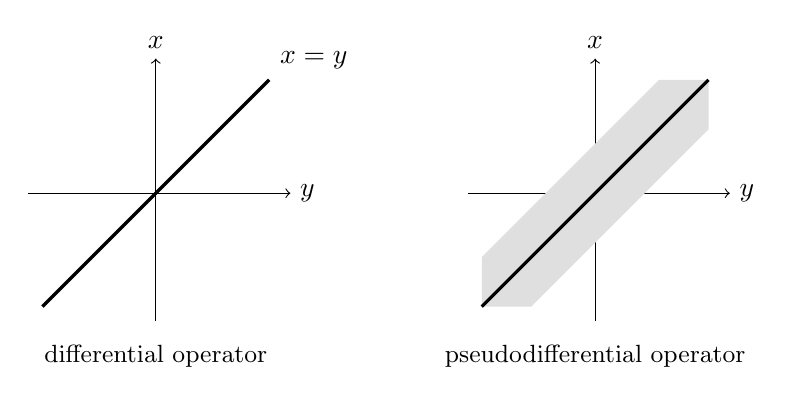
\begin{tikzpicture}[scale=0.9]
  \begin{scope}
    \draw[->] (-1.8,0)--(1.9,0) node[right]{$y$};
    \draw[->] (0,-1.8)--(0,1.9) node[above]{$x$};
    \draw[very thick] (-1.6,-1.6)--(1.6,1.6) node[above right]{$x=y$};
    \node at (0,-2.3) {\small differential operator};
  \end{scope}
  \begin{scope}[xshift=6.2cm]
    \draw[->] (-1.8,0)--(1.9,0) node[right]{$y$};
    \draw[->] (0,-1.8)--(0,1.9) node[above]{$x$};
    \fill[gray!25] (-1.6,-1.6)--(-1.6,-0.9)--(0.9,1.6)--(1.6,1.6)--(1.6,0.9)--(-0.9,-1.6)--cycle;
    \draw[very thick] (-1.6,-1.6)--(1.6,1.6);
    \node at (0,-2.3) {\small pseudodifferential operator};
  \end{scope}
\end{tikzpicture}
\caption{Supports and singularities of Schwartz kernels in the $(y,x)$-plane. A
differential operator, such as $\Id$ or $P(x,D)$, has kernel supported on the diagonal
$\{x=y\}$ (left). A pseudodifferential operator of \cref{ch:euclidean} has a kernel that
is still singular only on the diagonal, but is no longer supported there: it is smooth
off the diagonal and decays rapidly as $|x-y|\to\infty$ (right; the shading indicates
where the kernel is concentrated).}
\label{distributions:fig:kernels}
\end{figure}

\begin{question}
Where does the Fourier transform enter the proof of the kernel theorem, which is a
statement about operators and not about frequencies?
\end{question}
\begin{answer}
Only in \cref{distributions:lem:basic-est}. The Schwartz norms $\norm{\cdot}_k$ are not
Hilbert norms, so Riesz representation cannot be applied to them directly. After
applying $A_{N,M}^{-1}$, a Schwartz-norm estimate becomes a bound by
$\norm{\ang{\xi}^{-n}\hat\psi}_{L^2}$, a Hilbert norm. In that Hilbert space the point
evaluations $e_x$ are bounded, and this is what produces the continuous function $k$.
\end{answer}

%======================================================================
\section{Radial compactification}\label{distributions:sec:radial}

A real vector space $W$ of dimension $n$ is a smooth manifold, but $\CI(W)$ puts no
restriction on behaviour at infinity. A good way to describe functions with controlled
behaviour at infinity is to embed $W$ as a dense open subset of a compact manifold $X$,
possibly with boundary or corners, by a diffeomorphism onto its image. Restriction then
identifies $\CI(X)$ with a subspace of $\CI(W)$, since a smooth function is determined
by its values on a dense set. Several such compactifications exist. We construct them
first for $\R^n$ and then check how they behave under linear (and affine) changes of
coordinates. A compactification that is invariant under $\GL(n,\R)$ is well defined for
every vector space. For us the most important one is the \emph{radial
compactification}. Smooth functions on it are the classical symbols of order $0$, and
Schwartz functions are the smooth functions on it that vanish to infinite order at the
boundary.

\begin{discussion}
Why compactify at all? Estimates such as $|D^\alpha a(z)|\le C\ang{z}^{-|\alpha|}$, or
``rapid decay with all derivatives'', are conditions on the behaviour of a function at
infinity. On a compact manifold the analogous conditions are just smoothness, or
vanishing to infinite order, at a boundary. Compactifying turns asymptotic analysis at
infinity into local analysis near a boundary, where Taylor's formula and the other
tools of calculus apply. The price is that we must choose the compactification
carefully, so that the linear maps we care about extend smoothly.
\end{discussion}

\subsection{The one-point compactification and its defect}
\label{distributions:sec:one-point}
Identify $\R^n$ with the hyperplane $\{1\}\times\R^n\subset\R^{n+1}$, and let
$\Sphere^n\subset\R^{n+1}$ be the unit sphere. The line through the south pole $(-1,0)$
and $(1,z)$ is $t\mapsto(2t-1,tz)$. It meets $\Sphere^n$ again at
$t=4/(4+|z|^2)$, which gives the stereographic projection
\[
  P(z)=\Big(\frac{4-|z|^2}{4+|z|^2},\frac{4z}{4+|z|^2}\Big),\qquad
  P^{-1}(Z_0,Z)=\frac{2Z}{1+Z_0},\quad Z_0>-1.
\]
$P$ is a diffeomorphism of $\R^n$ onto $\Sphere^n$ minus the south pole. The
\emph{one-point compactification} $\oRC{\R^n}=\R^n\cup\{\infty\}$ is $\Sphere^n$ with this
identification. The reflection $Z_0\mapsto-Z_0$ corresponds to the inversion
$z\mapsto\iota(z)=4z/|z|^2$. Hence a function $f\in\CI(\R^n)$ extends smoothly to
$\oRC{\R^n}$ if and only if $f(\iota(w))$ extends smoothly across $w=0$. Orthogonal
transformations $O\in\mathrm{O}(n)$ lift to the diffeomorphisms $(Z_0,Z)\mapsto(Z_0,OZ)$.
General linear transformations do not.

\begin{proposition}\label{distributions:prop:one-point}
$G\in\GL(n,\R)$ extends to a $\mathcal{C}^1$ map of $\oRC{\R^n}$ fixing $\infty$ if and
only if $G$ is conformal, that is $G=cO$ with $c>0$ and $O\in\mathrm{O}(n)$. In
particular, for $n\ge2$ the scaling $(z_1,z')\mapsto(sz_1,z')$, $s\ne1$, does not
extend.
\end{proposition}
\begin{proof}
In the coordinate $w=\iota(z)$ near $\infty$, $G$ becomes
$h(w)=\iota(G\iota(w))=|w|^2Gw/|Gw|^2$ for $w\neq0$, with $h(0)=0$. If $G=cO$ then
$h(w)=c^{-1}Ow$, which is smooth. Conversely, suppose $h$ is differentiable at $0$.
Since $h(tw)=th(w)$ for $t>0$, we get
$h(w)=\lim_{t\downarrow0}h(tw)/t=h'(0)w$, so $h$ is linear, say $h(w)=Hw$. Then
$G^{-1}Hw=q(w)w$ with $q(w)=|w|^2/|Gw|^2$. So every vector is an eigenvector of
$G^{-1}H$, which is therefore a multiple $cI$ of the identity. Hence $q\equiv c$, that
is $|Gw|^2=c^{-1}|w|^2$, and $G$ is conformal.
\end{proof}

Thus the one-point compactification depends on a conformal structure on $W$, and not
only on its linear structure (\cref{distributions:ex:conformal}). It reappears in the
proof of the index theorem, but it is not the right compactification for symbols.

\begin{figure}[htbp]
\centering
\begin{tikzpicture}[scale=1.25,>=Latex]
  % one-point compactification
  \begin{scope}
    \draw (0,0) circle (1);
    \draw[thick] (-1.9,1)--(1.9,1) node[right]{\small $\{1\}\times\R^n$};
    \fill (0,-1) circle (0.04) node[below]{\small south pole $=\infty$};
    \coordinate (z) at (1.4,1);
    \draw[dashed] (0,-1)--(z);
    % intersection: t=4/(4+|z|^2) on line (-1,0)+t(2,z)  (drawn in (horizontal=z, vertical=X_0))
    \pgfmathsetmacro{\tpar}{4/(4+1.4*1.4)}
    \fill ($(0,-1)+\tpar*(1.4,2)$) circle (0.04);
    \fill (z) circle (0.04) node[above]{\small $z$};
    \node at (0,-1.75) {\small one-point: $\oRC{\R^n}$};
  \end{scope}
  % radial compactification
  \begin{scope}[xshift=5cm]
    \fill[gray!15] (-1,0) arc (180:0:1)--cycle;
    \draw (1,0) arc (0:180:1);
    \draw[very thick] (-1,0)--(1,0);
    \draw[thick] (-1.9,1)--(1.9,1) node[right]{\small $\{1\}\times\R^n$};
    \fill (0,0) circle (0.04) node[below]{\small $0$};
    \coordinate (z) at (1.4,1);
    \draw[dashed] (0,0)--(z);
    \pgfmathsetmacro{\rpar}{1/sqrt(1+1.4*1.4)}
    \fill ($\rpar*(1.4,1)$) circle (0.04);
    \fill (z) circle (0.04) node[above]{\small $z$};
    \draw[dashed] (0,0)--(-1.9,1);
    \pgfmathsetmacro{\rparb}{1/sqrt(1+1.9*1.9)}
    \fill ($\rparb*(-1.9,1)$) circle (0.04);
    \node[below] at (0.75,0) {\small $X_0=0$};
    \node at (0,-1.0) {\small radial: $\RC{\R^n}=\Sphere^n_+$};
    \node at (0,-1.4) {\small boundary $=$ sphere at infinity};
  \end{scope}
\end{tikzpicture}
\caption{Two compactifications of $\R^n$, drawn for $n=1$ with $\R^n$ placed at height
$X_0=1$. Left: stereographic projection from the south pole adds a single point
$\infty$. Right: projection from the origin maps $\R^n$ onto the open upper hemisphere,
and each direction $\omega$ in $\R^n$ acquires its own point at infinity on the
equator $\{X_0=0\}$.}
\label{distributions:fig:compactifications}
\end{figure}

\begin{question}
Why not use the one-point compactification for symbols? It is simpler, and it is a
smooth manifold without boundary.
\end{question}
\begin{answer}
For two reasons. First, \cref{distributions:prop:one-point} shows that general linear
changes of variables do not extend to it, while symbols must be invariant under them.
Second, the typical symbol $\xi/|\xi|$ (for $|\xi|>1$) has a different limit along each
ray, so it does not even extend continuously to a single point at infinity. The radial
compactification keeps one point at infinity for each direction, which is exactly what
homogeneous functions of degree $0$ need.
\end{answer}

\subsection{The radial compactification}
Instead of the south pole, project from the origin (\cref{distributions:fig:compactifications}). The ray from $0$ through $(1,z)$
meets the upper half of the unit sphere at the point
\begin{equation}\label{distributions:eq:RC}
  \mathrm{RC}\colon\R^n\ni z\longmapsto\Big(\frac1{\ang{z}},\frac z{\ang{z}}\Big)\in
  \Sphere^n_+=\{X=(X_0,X')\in\R^{n+1};\ X_0\ge0,\ |X|=1\}.
\end{equation}
This is a diffeomorphism onto the open hemisphere $\{X_0>0\}$, with inverse
$X\mapsto X'/X_0$. The closed hemisphere $\Sphere^n_+$ is a compact manifold with
boundary $\{X_0=0\}\cong\Sphere^{n-1}$, diffeomorphic to a closed ball.

\begin{definition}\label{distributions:def:RC}
The \emph{radial compactification} $\RC{\R^n}$ is $\Sphere^n_+$ with $\R^n$ identified
with its interior by $\mathrm{RC}$. Its boundary is the \emph{sphere at infinity}.
$\CI(\RC{\R^n})$ denotes the functions $f$ on $\R^n$ such that $f\circ\mathrm{RC}^{-1}$
extends to a smooth function on $\Sphere^n_+$, smooth up to the boundary. We write
$\dCI(\RC{\R^n})$ for the subspace of those that vanish to infinite order at the
boundary, with all derivatives.
\end{definition}

The function $\rho=X_0$, pulled back to $\ang{z}^{-1}$, is a \emph{boundary defining
function}: it is smooth, positive in the interior, and vanishes simply on the boundary.
Near the boundary there is a convenient product structure.

\begin{lemma}\label{distributions:lem:collar}
The map $z\mapsto(s,\omega)=(|z|^{-1},z/|z|)$, $|z|>1$, extends to a diffeomorphism of
a neighbourhood $\{X_0<|X'|\}$ of the boundary of $\RC{\R^n}$ onto
$[0,1)_s\times\Sphere^{n-1}$. Hence $f\in\CI(\R^n)$ is in $\CI(\RC{\R^n})$ if and only if
$f(z)=F(|z|^{-1},z/|z|)$ in $|z|>1$ for some $F\in\CI([0,1)\times\Sphere^{n-1})$. Moreover
\[
  \ang{z}^{-1}=s(1+s^2)^{-1/2},\qquad\frac{z}{\ang{z}}=(1+s^2)^{-1/2}\omega
\]
are in $\CI(\RC{\R^n})$.
\end{lemma}
\begin{proof}
In terms of $X$, $s=X_0/|X'|$ and $\omega=X'/|X'|$, which are smooth where $X'\ne0$. The
inverse is $X=(s,\omega)/(1+s^2)^{1/2}$, which is smooth on $[0,\infty)\times\Sphere^{n-1}$.
The region $|z|>1$ corresponds to $X_0<|X'|$, that is $s<1$.
\end{proof}

\begin{remark}\label{distributions:rem:RC-set}
As a set, $\RC{\R^n}=\R^n\sqcup\Sphere^{n-1}$, where the boundary point $(0,\omega)$ is
the limit of $\mathrm{RC}(t\omega)$ as $t\to\infty$, the ``end'' of the ray in
direction $\omega$. \Cref{distributions:lem:collar} shows that the smooth structure is
generated by the functions on $\R^n$ which, outside a compact set, are homogeneous of
degree $0$ (such as $z/|z|$), or homogeneous of degree $-1$ (such as $|z|^{-1}$). A
function homogeneous of degree $0$ for $|z|>1$ extends to $\RC{\R^n}$ with boundary
value its restriction to the unit sphere. A function homogeneous of negative integral
degree $-k$ is $s^k$ times such a function, and so vanishes at the boundary. For an
abstract vector space $W$ we set $\mathbb{S}W=(W\setminus0)/\R^+$ and
$\RC{W}=W\sqcup\mathbb{S}W$. The smooth structure is defined through any linear
isomorphism $W\to\R^n$, and it does not depend on the choice by
\cref{distributions:prop:affine} below.
\end{remark}

\subsection{Invariance}
\begin{proposition}\label{distributions:prop:affine}
Every affine map $T(z)=Gz+a$, $G\in\GL(n,\R)$, $a\in\R^n$, extends to a diffeomorphism
$\tilde T$ of $\RC{\R^n}$. Explicitly,
\[
  \tilde T(X)=\frac{MX}{|MX|},\qquad M(X_0,X')=(X_0,GX'+aX_0).
\]
In particular the radial compactification $\RC{W}$ of any real vector space is well
defined, and translations act on it smoothly.
\end{proposition}
\begin{proof}
$M$ is an invertible linear map of $\R^{n+1}$ that preserves $\{X_0>0\}$ and
$\{X_0=0\}$. If $X\in\Sphere^n_+$ then $MX\neq0$, so $\tilde T$ is a smooth map of a
neighbourhood of $\Sphere^n_+$ into $\Sphere^n_+$. Its inverse is the same construction
for $M^{-1}$, which corresponds to $T^{-1}$. Since $\mathrm{RC}(z)$ is a positive
multiple of $(1,z)$ and $M(1,z)=(1,Gz+a)$, we get
$\tilde T(\mathrm{RC}(z))=\mathrm{RC}(Tz)$.
\end{proof}

The infinitesimal version is also useful. It shows which vector fields on $\R^n$ extend
smoothly, and with what vanishing at infinity.

\begin{lemma}\label{distributions:lem:vf}
In the coordinates $(s,\omega)$ of \cref{distributions:lem:collar},
\[
  \pa_{z_j}=s\big(-\omega_j\,s\pa_s+W_j\big),\qquad
  z_i\pa_{z_j}=-\omega_i\omega_j\,s\pa_s+\omega_iW_j,
\]
where $W_j$ is the smooth vector field on $\Sphere^{n-1}$ given by orthogonal projection
of $e_j$ onto the tangent space, $W_j=\sum_k(\delta_{jk}-\omega_j\omega_k)\pa_{\omega_k}$.
Thus the linear vector fields $z_i\pa_{z_j}$ extend to smooth vector fields on
$\RC{\R^n}$ tangent to the boundary. The constant vector fields $\pa_{z_j}$ extend to
$\rho$ times smooth vector fields tangent to the boundary. Conversely, the radial
field $s\pa_s=-\sum_jz_j\pa_{z_j}$ and the rotation fields
$\Omega_{jk}=z_j\pa_{z_k}-z_k\pa_{z_j}$ span, over $\CI([0,1)\times\Sphere^{n-1})$, the
smooth vector fields tangent to the boundary near the boundary.
\end{lemma}
\begin{proof}
From $s=|z|^{-1}$ and $\omega=z/|z|$: $\pa_{z_j}s=-z_j|z|^{-3}=-s^2\omega_j$ and
$\pa_{z_j}\omega_k=s(\delta_{jk}-\omega_j\omega_k)$. This gives the first formula, and
the second follows on multiplying by $z_i=\omega_i/s$. The fields $\Omega_{jk}$ are
tangent to the spheres $|z|=\text{const}$, are homogeneous of degree $0$, and span the
tangent space of $\Sphere^{n-1}$ at every point.
\end{proof}

\subsection{Schwartz functions}
\begin{proposition}\label{distributions:prop:S-dCI}
Pull-back by $\mathrm{RC}$ identifies $\dCI(\RC{\R^n})$ with $\cS(\R^n)$, as sets and
as Fr\'echet spaces.
\end{proposition}
\begin{proof}
Both conditions are about behaviour in $|z|>1$, so we work in the collar
$[0,1)\times\Sphere^{n-1}$ and write $f(z)=F(s,\omega)$.

Suppose $F\in\dCI$. By \cref{distributions:lem:vf}, applying the first formula
repeatedly and using $V(s^pg)=s^p(V-p\omega_j)g$ for $V=-\omega_js\pa_s+W_j$, we get
$\pa_z^\beta f=s^{|\beta|}Q_\beta F$, where $Q_\beta$ is a differential operator with
smooth coefficients on $[0,1)\times\Sphere^{n-1}$. Also $z^\alpha=s^{-|\alpha|}\omega^\alpha$.
Since $F$ and all its derivatives vanish to infinite order at $s=0$,
$z^\alpha\pa^\beta f=s^{|\beta|-|\alpha|}\omega^\alpha Q_\beta F$ is bounded. So
$f\in\cS(\R^n)$.

Conversely, let $f\in\cS(\R^n)$. Every differential operator with smooth coefficients
on $[0,1)\times\Sphere^{n-1}$ is a combination, with smooth coefficients, of products of
$\pa_s$ and the $\Omega_{jk}$. On $s>0$ we have $\pa_s=-s^{-1}\sum_jz_j\pa_{z_j}=-|z|\sum_jz_j\pa_{z_j}$,
and $\Omega_{jk}$ has polynomial coefficients. Hence every derivative of $F$ is a
finite sum of smooth bounded coefficients times $|z|^p\,z^\alpha\pa_z^\beta f$, which is
$O(|z|^{-N})=O(s^N)$ for every $N$. A function on $(0,1)\times\Sphere^{n-1}$ all of
whose derivatives are $O(s^N)$ for all $N$ extends by zero to an element of
$\dCI([0,1)\times\Sphere^{n-1})$. Indeed, each derivative extends continuously by $0$,
and the difference quotient in $s$ at $s=0$ is $O(s^{N-1})\to0$, so by induction the
extension is $\mathcal{C}^k$ for all $k$ with vanishing derivatives at $s=0$. The
estimates in both directions are uniform, so the identification is a topological
isomorphism.
\end{proof}

Hence the dual space $\cSp(\R^n)$ is the dual of $\dCI(\RC{\R^n})$. The dual of $\dCI$
on a compact manifold with boundary is the space of \emph{extendible distributions},
so tempered distributions on $\R^n$ are exactly the extendible distributions on
$\RC{\R^n}$. This is one way of ``bringing infinity in''.

\subsection{Symbols as functions on the radial compactification}
\begin{proposition}\label{distributions:prop:symbols}
Let $a\in\CI(\RC{\R^n})$. Then:
\begin{enumerate}[label=(\roman*)]
\item $a\in\CI(\R^n)$ and $|D^\alpha a(z)|\le C_\alpha\ang{z}^{-|\alpha|}$ for all
  $\alpha$, so $a$ is a symbol of order $0$ in the sense of \cref{ch:euclidean};
\item there are $a_j\in\CI(\Sphere^{n-1})$ (the Taylor coefficients of $a$ at $s=0$)
  such that for every $N$
  \[
    r_N(z)=a(z)-\sum_{j<N}|z|^{-j}a_j(z/|z|)\quad\text{satisfies}\quad
    |D^\alpha r_N(z)|\le C_{N,\alpha}|z|^{-N-|\alpha|},\quad|z|>1;
  \]
\item for each polynomial $p$ of degree $m$, $\ang{z}^{-m}p\in\CI(\RC{\R^n})$, with
  boundary value $p_m(\omega)$, where $p_m$ is the homogeneous part of degree $m$.
\end{enumerate}
\end{proposition}
\begin{proof}
For (i), the proof of \cref{distributions:prop:S-dCI} gives
$\pa^\alpha a=s^{|\alpha|}Q_\alpha F$ in $|z|>1$, with $Q_\alpha F$ bounded. Since
$s\le2\ang{z}^{-1}$ there, this gives the estimate. In $|z|\le1$ it is trivial.
For (ii), Taylor's formula in $s$ gives
$F(s,\omega)=\sum_{j<N}s^ja_j(\omega)+s^NR_N(s,\omega)$ with $R_N$ smooth, and
$\pa^\alpha(s^NR_N)=s^{N+|\alpha|}Q'_\alpha R_N$ as before. For (iii),
$\ang{z}^{-m}z^\alpha=(z/\ang{z})^\alpha\ang{z}^{|\alpha|-m}$ is a product of components
of $X'$ and the power $X_0^{m-|\alpha|}$, so it is smooth. At $X_0=0$ only the terms with
$|\alpha|=m$ survive, and there $X'=\omega$.
\end{proof}

More generally, if $\rho\in\CI(\RC{W})$ is any boundary defining function, the space
\[
  \Symph{z}(W)=\rho^{-z}\CI(\RC{W}),\qquad z\in\C,
\]
is the space of \emph{classical} (or \emph{polyhomogeneous}) symbols of order $z$ on
$W$. It does not depend on the choice of $\rho$, since two boundary defining functions
differ by a positive smooth factor. By \cref{distributions:prop:affine} it is invariant
under affine changes of variables. Part (ii) of \cref{distributions:prop:symbols} is the
asymptotic expansion in homogeneous terms of decreasing degree that defines
polyhomogeneous symbols in \cref{ch:euclidean}. Using Borel's lemma one shows there
that, conversely, every symbol of order $0$ with such an expansion is in
$\CI(\RC{\R^n})$.

%======================================================================
\section{Further compactifications}\label{distributions:sec:other}

\subsection{The quadratic compactification}
Projecting the hemisphere $\Sphere^n_+$ onto its last $n$ coordinates gives a
homeomorphism onto the closed unit ball $\mathbb{B}^n$. Composing with $\mathrm{RC}$
gives the \emph{quadratic compactification}
\begin{equation}\label{distributions:eq:QRC}
  \mathrm{Q}\colon\R^n\ni z\longmapsto\frac z{\ang{z}}\in\mathbb{B}^n=\{y\in\R^n;\ |y|\le1\},
\end{equation}
a diffeomorphism onto the open ball. We write $\qRC{\R^n}$ for $\mathbb{B}^n$ with this
identification. The projection $\Sphere^n_+\to\mathbb{B}^n$ is smooth, but its inverse
$y\mapsto((1-|y|^2)^{1/2},y)$ is not smooth at $|y|=1$. So the identity of $\R^n$
extends to a smooth map $\RC{\R^n}\to\qRC{\R^n}$ but not conversely, and
$\CI(\qRC{\R^n})\subsetneq\CI(\RC{\R^n})$. Concretely, $\ang{z}^{-1}=(1-|y|^2)^{1/2}$ is
not smooth on $\qRC{\R^n}$. The function $1-|y|^2=\ang{z}^{-2}$ is a boundary defining
function there, and near the boundary $(t,\omega)=(|z|^{-2},z/|z|)$ are smooth
coordinates, which explains the name.

\begin{proposition}\label{distributions:prop:QRC}
\begin{enumerate}[label=(\roman*)]
\item Pull-back by $\mathrm{Q}$ identifies $\dCI(\qRC{\R^n})$, the smooth functions on
  $\R^n$ supported in $\mathbb{B}^n$, with $\cS(\R^n)$.
\item Every $G\in\GL(n,\R)$ extends to a diffeomorphism of $\qRC{\R^n}$, given by
  $y\mapsto Gy/(1-|y|^2+|Gy|^2)^{1/2}$.
\item For $n\ge2$ and $a\neq0$, the translation $z\mapsto z+a$ does not extend to a
  $\mathcal{C}^1$ map of $\qRC{\R^n}$.
\end{enumerate}
\end{proposition}
\begin{proof}
(i) Let $\pi(X)=X'$. If $g\in\dCI(\mathbb{B}^n)$ then $g\circ\pi\in\dCI(\Sphere^n_+)$,
because $\pi$ is smooth and maps the boundary to the boundary. Conversely, let
$f\in\dCI(\Sphere^n_+)$ and $g=f\circ\pi^{-1}$. A derivative of order $k$ of $g$ is a
sum of products of derivatives of $f$ at $\pi^{-1}(y)$ with derivatives of
$X_0=(1-|y|^2)^{1/2}$ of order at most $k$, which are $O(X_0^{1-2k})$. The derivatives
of $f$ are $O(X_0^N)$ for all $N$. So all derivatives of $g$ tend to $0$ at $|y|=1$, and
$g$ extended by $0$ is smooth. Now apply \cref{distributions:prop:S-dCI}.

(ii) With $y=z/\ang{z}$ we have $\ang{z}^2=(1-|y|^2)^{-1}$, so
$Gz/\ang{Gz}=Gy/(1-|y|^2+|Gy|^2)^{1/2}$. The denominator is positive on $\mathbb{B}^n$,
since $Gy\neq0$ when $|y|=1$, and the inverse is given by $G^{-1}$.

(iii) Let $\rho=(1-|y|^2)^{1/2}=\ang{z}^{-1}$. Since $\ang{z+a}^2=\ang{z}^2+2z\cdot a+|a|^2$,
the translation becomes
\[
  y\longmapsto\frac{y+\rho a}{(1+2\rho\,y\cdot a+\rho^2|a|^2)^{1/2}}
  =y+\rho\big(a-(y\cdot a)y\big)+\rho^2h(y,\rho),
\]
with $h$ smooth in $(y,\rho)$. Choose a unit vector $y_0\perp a$, which is possible as
$n\ge2$, and set $e=a/|a|$. Along $y=ty_0$, $t\uparrow1$, the $e$-component of the image
is $|a|\rho+\rho^2h_e$ with $\rho=(1-t^2)^{1/2}$. Its derivative in $t$ is unbounded as
$t\to1$, so the map is not $\mathcal{C}^1$ up to the boundary.
\end{proof}

Thus the quadratic compactification is well defined for a vector space, but not for an
affine space. In terms of vector fields, near the boundary
$z_i\pa_{z_j}=-2\omega_i\omega_j\,t\pa_t+\omega_iW_j$ is smooth, while
$\pa_{z_j}=t^{1/2}(-2\omega_j\,t\pa_t+W_j)$ is not. This is one reason to prefer the radial
compactification, on which translations act smoothly. The other is
\cref{distributions:prop:symbols}: classical symbols with terms of odd degree, such as
$\ang{z}^{-1}$, are smooth on $\RC{\R^n}$ but not on $\qRC{\R^n}$.

\subsection{Relation to the one-point compactification}
In the coordinate $w=\iota(z)=4z/|z|^2$ near $\infty\in\oRC{\R^n}$ we have
$w=4s\omega$ in terms of the coordinates of \cref{distributions:lem:collar}, and this
is smooth on $[0,1)\times\Sphere^{n-1}$. So the identity extends to a smooth map
\[
  \beta\colon\RC{\R^n}\longrightarrow\oRC{\R^n},
\]
which collapses the sphere at infinity to the point $\infty$ and is a diffeomorphism
elsewhere. In particular $\CI(\oRC{\R^n})\subset\CI(\RC{\R^n})$. Near the boundary,
$\beta$ is the introduction of polar coordinates $(s,\omega)\mapsto s\omega$ around
$\infty$. In the language of later chapters, $\RC{\R^n}$ is the \emph{blow-up}
$[\oRC{\R^n},\{\infty\}]$. In general, a manifold with boundary $X$ together with a smooth
map $\beta\colon X\to M$ is the blow-up of $M$ at $p$ if $\beta$ is a diffeomorphism of
$X\setminus\pa X$ onto $M\setminus\{p\}$, maps $\pa X$ to $p$, and polar coordinates
around $p$ (in some local coordinates) lift to a diffeomorphism of a neighbourhood of
$\pa X$ onto $[0,\epsilon)\times\Sphere^{n-1}$. This does not depend on the choice of local
coordinates (\cref{distributions:ex:polar}, and \cref{blowup:thm:invariance} for the
general statement). Blow-up of points and of more general submanifolds, and of manifolds
with corners, is developed systematically in \cref{ch:blowup}.

\subsection{Subspaces and relative compactifications}
\begin{proposition}\label{distributions:prop:inclusion}
If $V\subset W$ is a linear subspace, then the inclusion extends to a smooth embedding
$\RC{V}\hookrightarrow\RC{W}$, and likewise $\qRC{V}\hookrightarrow\qRC{W}$. Every
injective linear map $V\to W$ extends to a smooth map $\RC{V}\to\RC{W}$.
\end{proposition}
\begin{proof}
By \cref{distributions:prop:affine} we may choose coordinates with $V=\R^k\times\{0\}$.
Then $\mathrm{RC}_n(v,0)=(\ang{v}^{-1},v/\ang{v},0)$, which is the standard embedding
$\Sphere^k_+\hookrightarrow\Sphere^n_+$ composed with $\mathrm{RC}_k$. The quadratic case is
the same. An injective linear map is an isomorphism onto its image followed by an
inclusion.
\end{proof}

Linear maps that are not injective do not extend in general
(\cref{distributions:ex:projection}): the points at infinity ``do not know where to go''.
The remedy is to compactify relative to a subspace. Let $V\subset W$ and choose a
complement $U$, so $W=V\times U$, together with Euclidean metrics on $V$ and $U$. Consider
\begin{equation}\label{distributions:eq:relRC}
  R_V\colon W\ni(v,u)\longmapsto\big(\mathrm{RC}_U(u),\ \mathrm{RC}_V(v/\ang{u})\big)
  \in\RC{U}\times\RC{V}.
\end{equation}
Explicitly, $R_V(v,u)=(t,u',s,v')$ with
\[
  t=\frac1{\ang{u}},\quad u'=\frac u{\ang{u}},\quad
  s=\frac{\ang{u}}{(1+|u|^2+|v|^2)^{1/2}},\quad v'=\frac v{(1+|u|^2+|v|^2)^{1/2}},
\]
satisfying $t^2+|u'|^2=1=s^2+|v'|^2$. Here we used
$\ang{v/\ang{u}}=(1+|u|^2+|v|^2)^{1/2}/\ang{u}$. The map $(v,u)\mapsto(v/\ang{u},u)$ is a
diffeomorphism of $W$, so $R_V$ is a diffeomorphism onto the interior of the compact
manifold with corners $\RC{U}\times\RC{V}$, with inverse $(t,u',s,v')\mapsto(v'/(st),u'/t)$.
We write $\relRC{V}{W}$ for $\RC{U}\times\RC{V}$ with this identification, and call it the
\emph{radial compactification of $W$ relative to $V$}. \Cref{distributions:fig:relative}
shows the simplest case.

\begin{figure}[htbp]
\centering
\begin{tikzpicture}[scale=1.2,>=Latex]
  \begin{scope}
    \fill[gray!15] (-1,-1) rectangle (1,1);
    \draw[thick] (-1,-1)--(1,-1) (-1,1)--(1,1);
    \draw[very thick] (-1,-1)--(-1,1) (1,-1)--(1,1);
    \node[below] at (0,-1) {\small $\{u'=-1\}$};
    \node[above] at (0,1) {\small $\{u'=+1\}$};
    \node[left,align=right] at (-1,0) {\small front\\[-0.6ex]\small face};
    \node[right,align=left] at (1,0) {\small front\\[-0.6ex]\small face};
    \draw[->] (-0.5,0)--(0.6,0) node[right]{\small $v$};
    \draw[->] (0,-0.5)--(0,0.6) node[above]{\small $u$};
    \node at (0,-1.75) {\small $\relRC{V}{W}=\RC{U}\times\RC{V}$};
  \end{scope}
  \draw[->] (2.3,0)--(3.4,0) node[midway,above]{\small $\beta$};
  \begin{scope}[xshift=5.2cm]
    \fill[gray!15] (0,0) circle (1);
    \draw[thick] (0,0) circle (1);
    \fill (1,0) circle (0.06) node[right]{\small $+\mathbb{S}V$};
    \fill (-1,0) circle (0.06) node[left]{\small $-\mathbb{S}V$};
    \draw[->] (-0.5,0)--(0.6,0) node[above]{\small $v$};
    \draw[->] (0,-0.5)--(0,0.6) node[above]{\small $u$};
    \node at (0,-1.75) {\small $\RC{W}$};
  \end{scope}
\end{tikzpicture}
\caption{The relative compactification for $W=\R^2$, $V=\R\times\{0\}$ and $U=\{0\}\times\R$.
The square $\RC{U}\times\RC{V}$ maps onto the disc $\RC{W}$ by a map $\beta$ extending
the identity of $W$. The faces $\{s=0\}$ (heavy vertical sides), where $|v|\to\infty$
with $u$ bounded, collapse to the two points $\pm\mathbb{S}V$ of the sphere at infinity
of $V$; the other two sides map to the two arcs of the circle. This is the blow-up
$[\RC{W},\mathbb{S}V]$ of \cref{distributions:rem:blowup}.}
\label{distributions:fig:relative}
\end{figure}

\begin{proposition}\label{distributions:prop:relative}
Every affine map of $W$ whose linear part maps $V$ into itself extends to a
diffeomorphism of $\relRC{V}{W}$. In particular $\relRC{V}{W}$ does not depend on the
choice of complement $U$ or of the metrics. The short exact sequence
$0\to V\to W\to W/V\to0$ extends to smooth maps
\[
  \RC{V}\longrightarrow\relRC{V}{W}\longrightarrow\RC{W/V}.
\]
If $A\colon V\to W$ is any linear map with null space $N$, then $A$ extends to a smooth
map $\relRC{N}{V}\to\RC{W}$.
\end{proposition}
\begin{proof}
An affine map preserving the direction $V$ has the form
$T(v,u)=(Gv+Su+a,\,Hu+b)$, with $G\in\GL(V)$, $H\in\GL(U)$, $S\colon U\to V$ linear,
$a\in V$ and $b\in U$. In the coordinates $(\nu,u)=(v/\ang{u},u)$ it becomes
\[
  (\nu,u)\longmapsto\Big(c(u)\big(G\nu+S\tfrac u{\ang{u}}+a\ang{u}^{-1}\big),\ Hu+b\Big),\qquad
  c(u)=\frac{\ang{u}}{\ang{Hu+b}}.
\]
By \cref{distributions:prop:affine}, $u\mapsto Hu+b$ extends to a diffeomorphism of
$\RC{U}$, and $\ang{Hu+b}^{-1}$ is the pull-back of the boundary defining function
$\ang{u}^{-1}$ under this map. Hence $c$ is a positive function in $\CI(\RC{U})$. The
functions $u/\ang{u}$ and $\ang{u}^{-1}$ are also in $\CI(\RC{U})$. Thus the first
component is an affine map of $V$, with invertible linear part, depending smoothly on the
parameter $p\in\RC{U}$. The formula of \cref{distributions:prop:affine}, with $M$
depending smoothly on $p$, shows that it extends smoothly to
$\RC{U}\times\RC{V}$. The same holds for the inverse. Changing the complement or the
metrics is such a linear map, so $\relRC{V}{W}$ does not depend on these choices.

The inclusion $v\mapsto(v,0)$ becomes $v\mapsto(\mathrm{RC}_U(0),\mathrm{RC}_V(v))$,
which extends to $\RC{V}\cong\{\mathrm{RC}_U(0)\}\times\RC{V}$. The projection
$(v,u)\mapsto u$, with $U\cong W/V$, extends as the projection
$\RC{U}\times\RC{V}\to\RC{U}$. Finally, write $A$ as the projection $V\to V/N$ followed
by the injective map $V/N\to W$ induced by $A$, and use the first part of this
proposition together with \cref{distributions:prop:inclusion}.
\end{proof}

\begin{remark}\label{distributions:rem:blowup}
In the trivial cases $V=\{0\}$ and $V=W$ the relative compactification reduces to
$\RC{W}$ (\cref{distributions:ex:trivial}). For a non-trivial subspace, $\relRC{V}{W}$
is canonically the blow-up $[\RC{W},\mathbb{S}V]$ of $\RC{W}$ along the sphere at
infinity of $V$, which is a submanifold of the boundary. Similarly, for a product
$W=V\times U$ the identity map extends to neither $\RC{V}\times\RC{U}\to\RC{W}$ nor its
inverse. However, the doubly-relative compactification
(\cref{distributions:ex:doubly}) is canonically both $[\RC{V\times U};\mathbb{S}U,\mathbb{S}V]$
and $[\RC{V}\times\RC{U};\mathbb{S}V\times\mathbb{S}U]$. These identifications are
proved in \cref{ch:blowup}: the first in \cref{blowup:thm:relative} (where $\mathbb{S}V$
is shown to be a p-submanifold of $\RC{W}$, of codimension $\dim W-\dim V+1$), the second
in \cref{blowup:prop:doubly}.
\end{remark}

%======================================================================
\section{Exercises}\label{distributions:sec:exercises}

\begin{exercise}\label{distributions:ex:taylor}
Suppose $\phi\colon\R^n\to\C$ is such that for each $\bar x\in\R^n$ and each $k\in\N_0$
there are $\epsilon_k>0$ and a polynomial $p_k(x;\bar x)$ with
$|\phi(x)-p_k(x;\bar x)|\le\epsilon_k^{-1}|x-\bar x|^{k+1}$ for $|x-\bar x|\le\epsilon_k$.
Must $\phi$ be infinitely differentiable? (Consider
$\phi(x)=e^{-1/x^2}\sin(e^{1/x^2})$ on $\R$.)
\end{exercise}

\begin{exercise}\label{distributions:ex:exp-cos}
Show that $u(x)=e^x\cos(e^x)$ is a tempered distribution on $\R$, in the sense that
there is $T\in\cSp(\R)$ with $T(\phi)=\int u\phi\,dx$ for all $\phi\in\CIc(\R)$. Show
that $T$ is unique. (Write $u$ as the derivative of a bounded function.) Note that
$\int u\phi\,dx$ need not converge absolutely for $\phi\in\cS(\R)$.
\end{exercise}

\begin{exercise}\label{distributions:ex:metric}
Show that $d$ in \eqref{distributions:eq:metric} is a metric on $\cS(\R^n)$. (If
$\norm{\cdot}$ is a norm, show that
$\frac{\norm{u+v}}{1+\norm{u+v}}\le\frac{\norm{u}}{1+\norm{u}}+\frac{\norm{v}}{1+\norm{v}}$.)
\end{exercise}

\begin{exercise}\label{distributions:ex:cauchy}
Show that a sequence $\phi_j\in\cS(\R^n)$ is Cauchy, respectively converges to $\phi$,
for $d$ if and only if it is Cauchy, respectively converges to $\phi$, for each norm
$\norm{\cdot}_k$.
\end{exercise}

\begin{exercise}\label{distributions:ex:bilinear}
Show that a bilinear map $B\colon\cS(\R^n)\times\cS(\R^p)\to\C$ is (jointly) continuous
if and only if $|B(\phi,\psi)|\le C\norm{\phi}_N\norm{\psi}_N$ for some $C$ and $N$.
Combined with \cref{distributions:lem:joint}, this shows that separate continuity
implies joint continuity.
\end{exercise}

\begin{exercise}\label{distributions:ex:restriction}
Show that the restriction map $\pi_k^*\colon\cS(\R^n)\to\cS(\R^k)$ is continuous and
surjective.
\end{exercise}

\begin{exercise}\label{distributions:ex:gaussian-contour}
Give a second proof of \cref{distributions:lem:gaussian}. For $n=1$ write
$\int e^{-ix\xi}e^{-x^2}dx=e^{-\xi^2/4}\int e^{-(x+\frac i2\xi)^2}dx$, interpret the
integral as a contour integral, and shift the contour to $\operatorname{Im}x=-\xi/2$.
\end{exercise}

\begin{exercise}\label{distributions:ex:L2}
Show that \eqref{distributions:eq:Tphi} makes sense for $\phi\in L^2(\R^n)$, and that the
resulting map $L^2(\R^n)\to\cSp(\R^n)$ is injective.
\end{exercise}

\begin{exercise}\label{distributions:ex:sobolev}
(A weak Sobolev embedding.)
\begin{enumerate}[label=(\alph*)]
\item Show that if $f\in L^1(\R^n)$ then
  $v(x)=\int_{-\infty}^{x_1}\cdots\int_{-\infty}^{x_n}f(t)\,dt$ is bounded and continuous
  and $D_1\cdots D_nv=(-i)^nf$ in $\cSp(\R^n)$. Show that
  $(1+|x|)^{-n-1}L^2(\R^n)\subset L^1(\R^n)$.
\item Show that if $u\in\cSp(\R^n)$ and $\ang{\xi}^s\hat u\in L^2(\R^n)$ for some
  $s>n/2+k$, then $u\in\mathcal{C}^k(\R^n)$ and $D^\alpha u$ is bounded and continuous for
  $|\alpha|\le k$.
\end{enumerate}
\end{exercise}

\begin{exercise}\label{distributions:ex:support}
Show that for $\phi\in\cS(\R^n)$ (indeed for $\phi$ continuous and polynomially bounded),
the support of $T_\phi$ in the sense of \cref{distributions:def:support} is the closure
of $\{x;\ \phi(x)\neq0\}$. Show that $\supp\delta=\{0\}$.
\end{exercise}

\begin{exercise}\label{distributions:ex:peetre}
Show that a differential operator $P$ with coefficients in $\CIb(\R^n)$ is \emph{local}:
$\supp(Pu)\subset\supp u$ for all $u\in\cSp(\R^n)$. The converse, for a linear operator
$P\colon\cS(\R^n)\to\cS(\R^n)$ with $\supp(Pu)\subset\supp u$ and (for simplicity)
$\supp(Pu)\subset K$ for a fixed compact $K$, is Peetre's theorem. How would you try to
prove it? (No full proof required.)
\end{exercise}

\begin{exercise}\label{distributions:ex:delta-rep}
Find a bounded continuous function $w$ on $\R$ with $\delta=(1+D^2)w$, as predicted by
\cref{distributions:thm:structure}. (Try $w=\frac12e^{-|x|}$.) Can $\delta$ be written
as $Dw$ with $w$ bounded and continuous?
\end{exercise}

\begin{exercise}\label{distributions:ex:exterior}
Use \cref{distributions:thm:kernel} to show that for $u\in\cSp(\R^n)$ and
$v\in\cSp(\R^m)$ there is a unique $u\boxtimes v\in\cSp(\R^{n+m})$ with
$(u\boxtimes v)(\phi\boxtimes\psi)=u(\phi)v(\psi)$.
\end{exercise}

\begin{exercise}\label{distributions:ex:conformal}
Formulate precisely the notion of a conformal structure on a real vector space $W$
(a Euclidean metric up to positive multiples). Show that the one-point
compactification of $W$ depends only on such a structure. If $V\subset W$ carries the
induced conformal structure, show that the inclusion extends to a smooth map
$\oRC{V}\to\oRC{W}$.
\end{exercise}

\begin{exercise}\label{distributions:ex:qrc-abstract}
Show that the quadratic compactification can be defined for any real vector space, and
that as a set it is again $W\sqcup\mathbb{S}W$, with a different smooth structure. (Use
\cref{distributions:prop:QRC}(ii).)
\end{exercise}

\begin{exercise}\label{distributions:ex:projection}
Show that the projection $\R^2\ni(z_1,z_2)\mapsto z_1\in\R$ does not extend to a
continuous map $\RC{\R^2}\to\RC{\R}$. (Consider the curves $z=(c,t)$, $t\to\infty$.)
Show more generally that a non-zero linear map between vector spaces of positive
dimension extends continuously to the radial (or quadratic) compactifications if and only if it is
injective.
\end{exercise}

\begin{exercise}\label{distributions:ex:trivial}
Show from \eqref{distributions:eq:relRC} that $\relRC{\{0\}}{W}$ and $\relRC{W}{W}$ are
both canonically $\RC{W}$.
\end{exercise}

\begin{exercise}\label{distributions:ex:doubly}
(Doubly-relative compactification.) For $W=V\times U$ with metrics on $V$ and $U$,
consider
\[
  W\ni(v,u)\longmapsto\Big(\frac{1}{\ang{u}},\frac{1}{\ang{v}},
  \frac{\ang{u}}{\ang{(u,v)}},\frac{\ang{v}}{\ang{(u,v)}},\frac{v}{\ang{v}},
  \frac{(v,u)}{\ang{(u,v)}},\frac{u}{\ang{u}}\Big)\in\R^4\times V\times W\times U.
\]
Show that this is a diffeomorphism onto its image, and that the closure of the image is
a compact manifold with corners. It has three boundary hypersurfaces if
$\dim U,\dim V\ge2$. Denote it by $\relRC{U,V}{U\times V}$. Show that translations, and
linear maps preserving both $U$ and $V$, lift to diffeomorphisms. Show that the
inclusions of $\RC{U}$ and $\RC{V}$ extend smoothly, and that the identity of $W$
extends to smooth maps from $\relRC{U,V}{U\times V}$ to both $\RC{U\times V}$ and
$\RC{U}\times\RC{V}$. Draw a picture for $\dim U=\dim V=1$. (The identification of this
space with two iterated blow-ups is \cref{blowup:prop:doubly}; compare
\cref{blowup:fig:octagon}.)
\end{exercise}

\begin{exercise}\label{distributions:ex:polar}
Show that a change of local coordinates fixing $0\in\R^n$ induces a diffeomorphism of
$[0,\epsilon)\times\Sphere^{n-1}$, for some $\epsilon>0$, under polar coordinates
$(r,\omega)\mapsto r\omega$. (Treat linear changes first, using
\cref{distributions:prop:affine}. Then reduce to the case where the Jacobian at $0$ is
the identity.) Conclude that the blow-up of a point is well defined. (The general form of
this statement, for submanifolds and with the action on the front face, is
\cref{blowup:thm:invariance}.)
\end{exercise}

\section*{Notes}
This chapter merges Chapter~1 of \emph{Introduction to Microlocal Analysis} with Lecture~1
(and its addenda) of \emph{Lectures on Pseudodifferential Operators}. The ``two big
theorems'' were only stated in the original, with outlines of proofs in the problems.
Here they are proved in full, using a single estimate
(\cref{distributions:lem:basic-est}) and a Riesz representation argument in place of
the Hilbert--Schmidt argument suggested originally. Separate continuity is upgraded to
joint continuity by a Baire category argument, and uniqueness of the kernel uses the
density of tensor products. The classification of distributions supported at a point
is proved in all dimensions. Both compactification discussions have been unified around
the explicit formulae \eqref{distributions:eq:RC} and
\cref{distributions:prop:affine}, which replace the Lie algebra arguments of the
original. The relative compactification is written as a product
$\RC{U}\times\RC{V}$ by the change of variables $v\mapsto v/\ang{u}$. For the
kernel theorem and the structure of distributions see \cite[Chapter~5 and
\S7.1]{Hormander-I} and \cite{Friedlander}. Compactifications, blow-ups and manifolds
with corners are treated systematically in Melrose's work on the $b$-calculus, see
\cite{Melrose-APS}.
